\documentclass[10pt, conference, compsocconf]{beamer}

\usepackage[T1]{fontenc}
\usepackage{CJKutf8}

\usepackage[unicode=true,pdfusetitle,
 bookmarks=true,bookmarksnumbered=false,bookmarksopen=false,
 breaklinks=false,pdfborder={0 0 1},backref=false,colorlinks=false]
 {}

%\documentclass{beamer}
\usepackage{BeamerColor}
\usepackage{times}  % fonts are up to you
\usepackage{graphicx}
\usepackage{setspace}
\usepackage{cite}
\usepackage{amsmath,epsfig}
\usepackage{booktabs}
\usepackage{epstopdf}
\usepackage{algorithmic}
\usepackage{graphics}
\usepackage{midfloat}
%\usepackage{listings}
\usepackage[ruled]{algorithm2e}
\usepackage{multirow}
\usepackage{tabularx}
\usepackage{textpos}

% for themes, etc.
\mode<presentation>
{ 
	\usecolortheme[named=SkyBlue4]{structure}
	\usetheme{Madrid}
	\usefonttheme[onlysmall]{structurebold}
 }


\CJKencfamily{UTF8}{bkai} % 使用標楷體


\AtBeginDocument{%
    \begin{CJK}{UTF8}{bkai}} % 使用標楷體
    \AtEndDocument{%
    \clearpage\end{CJK}}


\begin{document}
\begin{CJK}{UTF8}{}%
% these will be used later in the title page
\title{基於即時情緒分析之心靈陪伴系統}
\author{
賴詩雨, 蔡怡君, 龐渝庭, 蔡昕云, 吳悅琳 \\
\vspace{5mm}
AI Comforter\\
%\date{June 29, 2016}
}


% have this if you'd like a recurring outline
\AtBeginSection[]  % "Beamer, do the following at the start of every section"
{
\begin{frame}<beamer> 
\frametitle{大綱} % make a frame titled "Outline"
\tableofcontents[currentsection]  % show TOC and highlight current section
\end{frame}
}

%\begin{document}

\addtobeamertemplate{frametitle}{}{%
\begin{textblock*}{100mm}(.88\textwidth,-0.85cm)

\includegraphics[width=1.5cm]{./Figures/AI_Comforter_5.png}
\end{textblock*}}

% this prints title, author etc. info from above
\begin{frame}
\titlepage
\raggedleft 
\includegraphics[width=1.5cm]{./Figures/AI_Comforter_5.png} ~
\raggedleft 
\includegraphics[width=0.9cm]{./Figures/yzu-logo.png}
\end{frame}



\begin{frame}
\frametitle{大綱}
  \tableofcontents
\end{frame}

\section{背景介紹}
\begin{frame}
\frametitle{背景介紹}
%步調快

\begin{itemize}
\item \Large 現代人生活步調快
\end{itemize}
%。現代社會生活步調快速,大部分的人為了工作或課業等外在的壓力,身心常處於緊張又忙碌的狀態,造成生活作息不正常,甚至引起許多身體與心理方面的疾病。


\begin{figure}[!t]
\begin{center}
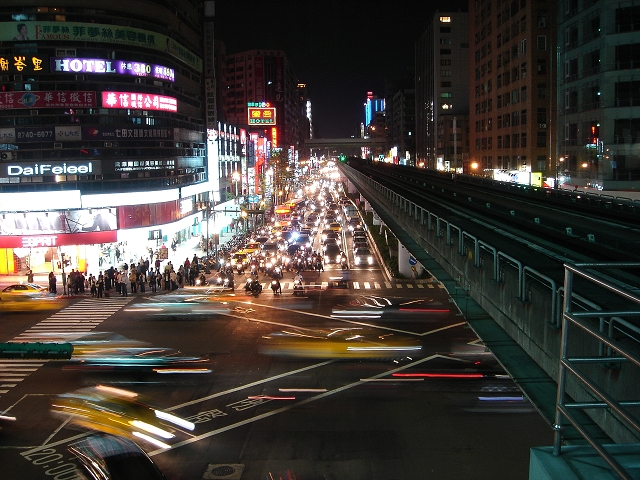
\includegraphics[width=7cm]{./Figures/0.jpg}
\end{center}
\end{figure}

\end{frame}

\begin{frame}
\frametitle{背景介紹}
%易生病

\begin{itemize}
\item \Large 容易產生疾病  
\end{itemize}
\vspace{5mm}
\begin{figure}[!t]
\begin{center}
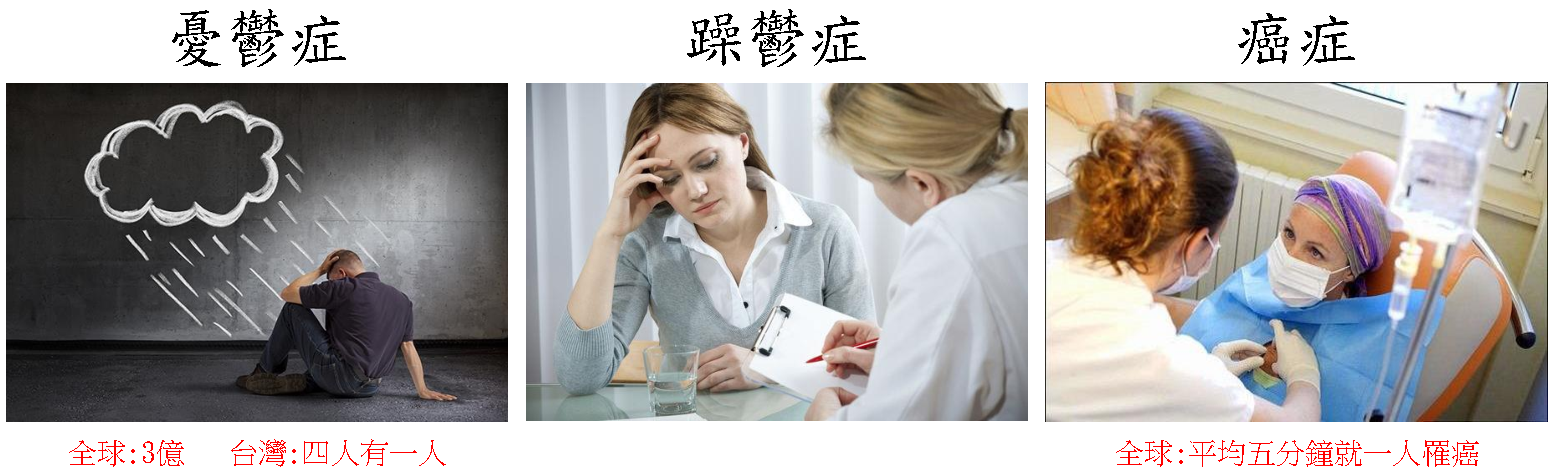
\includegraphics[width=12cm]{./Figures/fig_disease.pdf}
\end{center}
%\caption{\scriptsize List of gaming applications}
\label{fig:device}
\end{figure}

\end{frame}


\begin{frame}
\frametitle{背景介紹}
%因素

\begin{itemize}
\item \Large正常接受治療下,疾病控制和康復的因素
\end{itemize}
\vspace{5mm}
\begin{figure}[!t]
\begin{center}

\includegraphics[width=11.5cm]{./Figures/fig_doctor.pdf}
\end{center}
\end{figure}

\end{frame}

\section{創新\&創意}
%研究證明

\begin{frame}
\frametitle{創新\&創意}

\begin{itemize}
\item \Large研究證明 : 好的情緒幫助治療疾病
\end{itemize}
\vspace{5mm}
\begin{figure}[!t]
\begin{center}
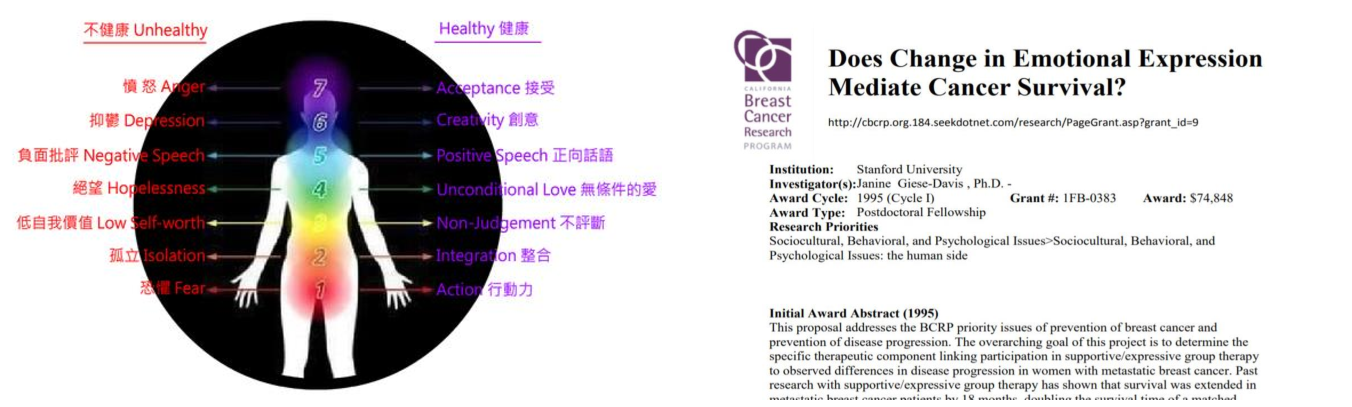
\includegraphics[width=12.5cm]{./Figures/fig_theory.pdf}
\end{center}

\end{figure}
\end{frame}

\begin{frame}
\frametitle{創新\&創意}
%親朋好友

\begin{itemize}
\item\Large穩定情緒方法
\end{itemize}

\begin{columns}
\column{.4\textwidth}
\begin{itemize}
\item[-] \large\bf親朋好友
\vspace{5mm}
\end{itemize}
\begin{itemize}
\item[*]  不想和認識的人說\\
\vspace{5mm}
\item[*]  不能感同身受 : 心情變更糟\\
\vspace{5mm}
\textcolor{red}{不專業}
\vspace{5mm}
\end{itemize}
\column{.6\textwidth}
\begin{figure}[!t]
\begin{flushright}
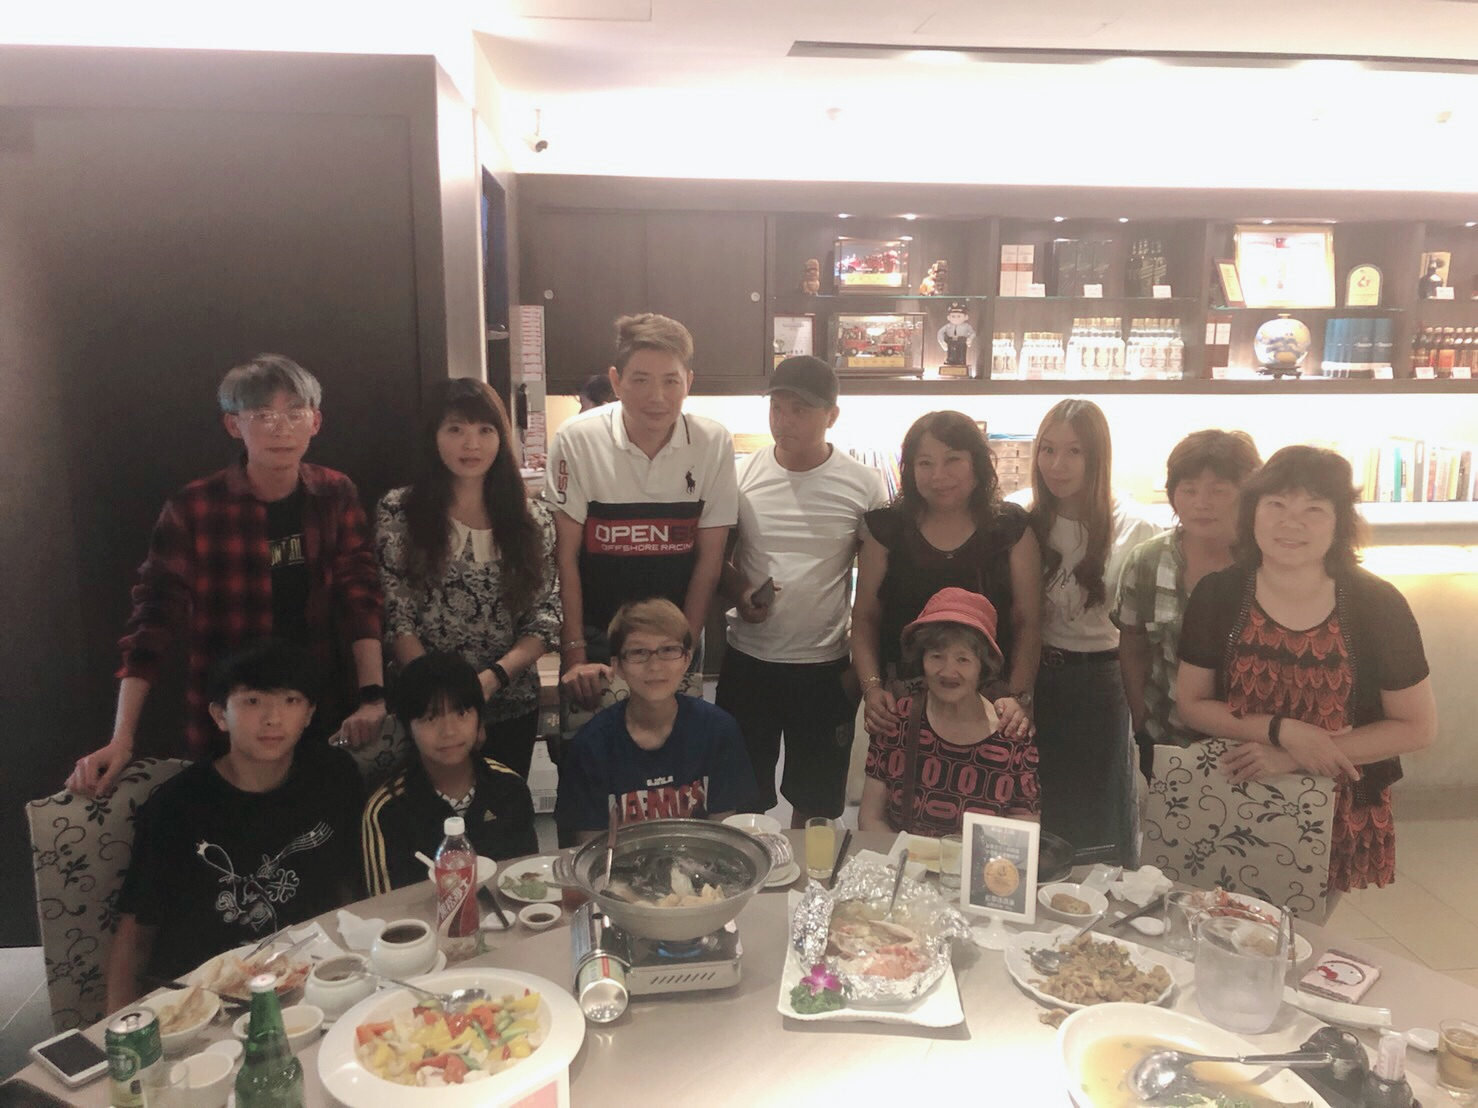
\includegraphics[width=0.9\textwidth]{Figures/9.jpg}
\end{flushright}
\end{figure}
\end{columns}

\end{frame}

\begin{frame}
\frametitle{創新\&創意}
%心理諮詢師

\begin{itemize}
\item\Large穩定情緒方法
\end{itemize}

\begin{columns}
\column{.4\textwidth}
\begin{itemize}
\item[-] \large\bf心理諮詢師
\vspace{5mm}
\end{itemize}
\begin{itemize}
\item[*]  要預約 : 不能及時緩解當下情緒\\
\vspace{2mm}
\textcolor{red}{不即時}
\vspace{5mm}
\item[*]  昂貴且單次計算費用 : NT\$ 2500 / 50 min\\
\vspace{2mm}
\textcolor{red}{沒有後續追蹤}
\end{itemize}
\column{.6\textwidth}
\begin{figure}[!t]
\begin{flushright}
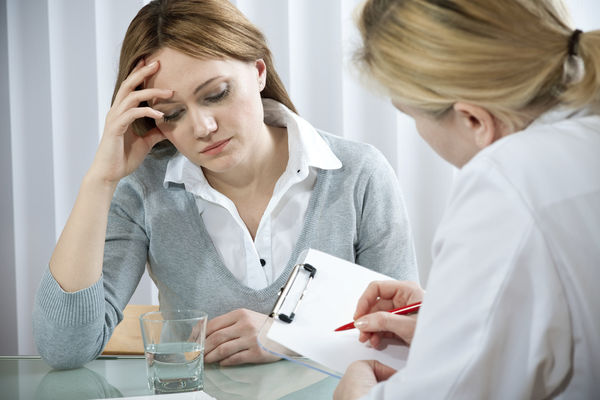
\includegraphics[width=0.9\textwidth]{Figures/3.jpg}
\end{flushright}
\end{figure}
\end{columns}

\end{frame}


\begin{frame}
\frametitle{創新\&創意}
%比較表

\begin{itemize}
\item\Large穩定情緒方法比較
\end{itemize}
\vspace{8mm}
\begin{table}[!h]
\small
\centering
\resizebox{0.9\textwidth}{!}{
\begin{tabular}{|c|c|c|c|}  
\hline
特性		&專業性	&即時性  &後續追蹤 \\ \hline
\hline
心理諮詢師	& O 	& X	& X		\\ \hline
親朋好友 	& X	& O	& Δ 	\\ \hline
本系統    	& O	& O	& O 	\\ \hline
\end{tabular}}
\label{tab:accuracy}
\end{table}

\end{frame}

\begin{frame}
\frametitle{創新\&創意}
%作品特色

\begin{itemize}
\item\Large基於即時情緒分析之心靈陪伴系統
\end{itemize}

\begin{columns}
\column{.5\textwidth}
\begin{itemize}
\item[-] \Large\bf 即時分析情緒
\vspace{5mm}
\item[-] \Large\bf 專業的緩和機制
\vspace{5mm}
\item[-] \Large\bf 後端平台做分析追蹤
\end{itemize}

\column{.5\textwidth}
\begin{figure}[!t]
\begin{flushright}
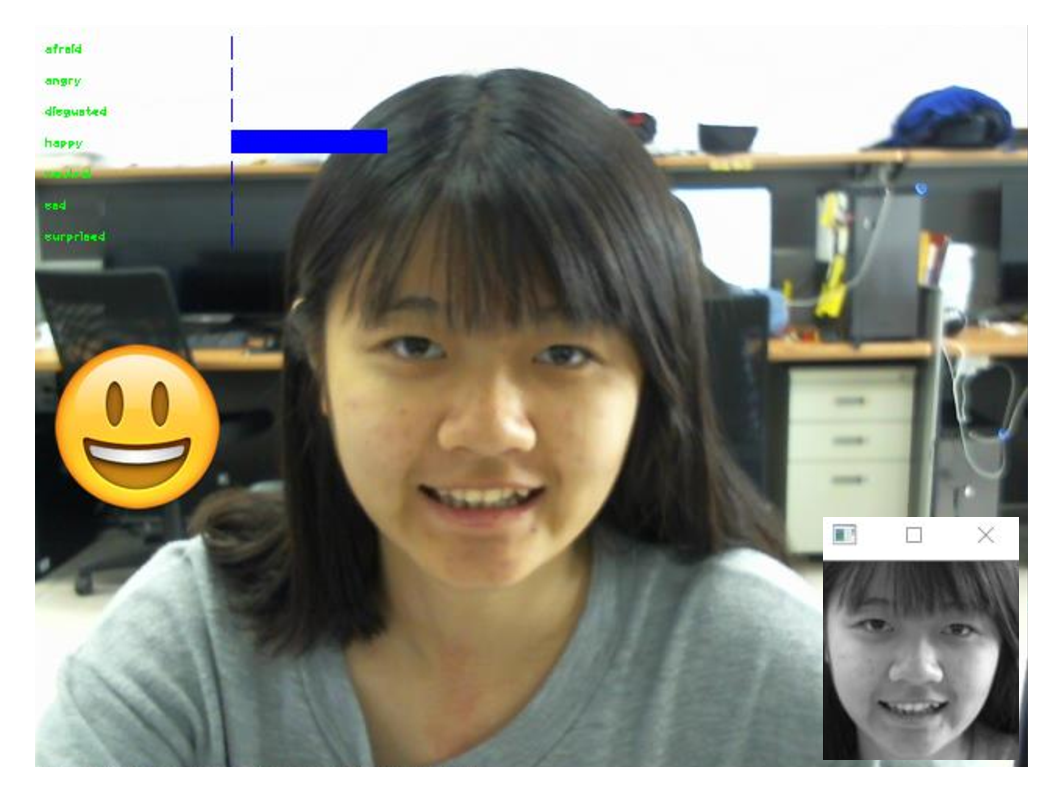
\includegraphics[width=0.9\textwidth]{Figures/DetectResult.pdf}
\end{flushright}
\end{figure}
\end{columns}

\end{frame}


\section{作品介紹}

\begin{frame}
\frametitle{作品介紹}
%系統架構
\begin{itemize}
\item \Large系統架構
\end{itemize}

\begin{figure}[!t]
\begin{center}
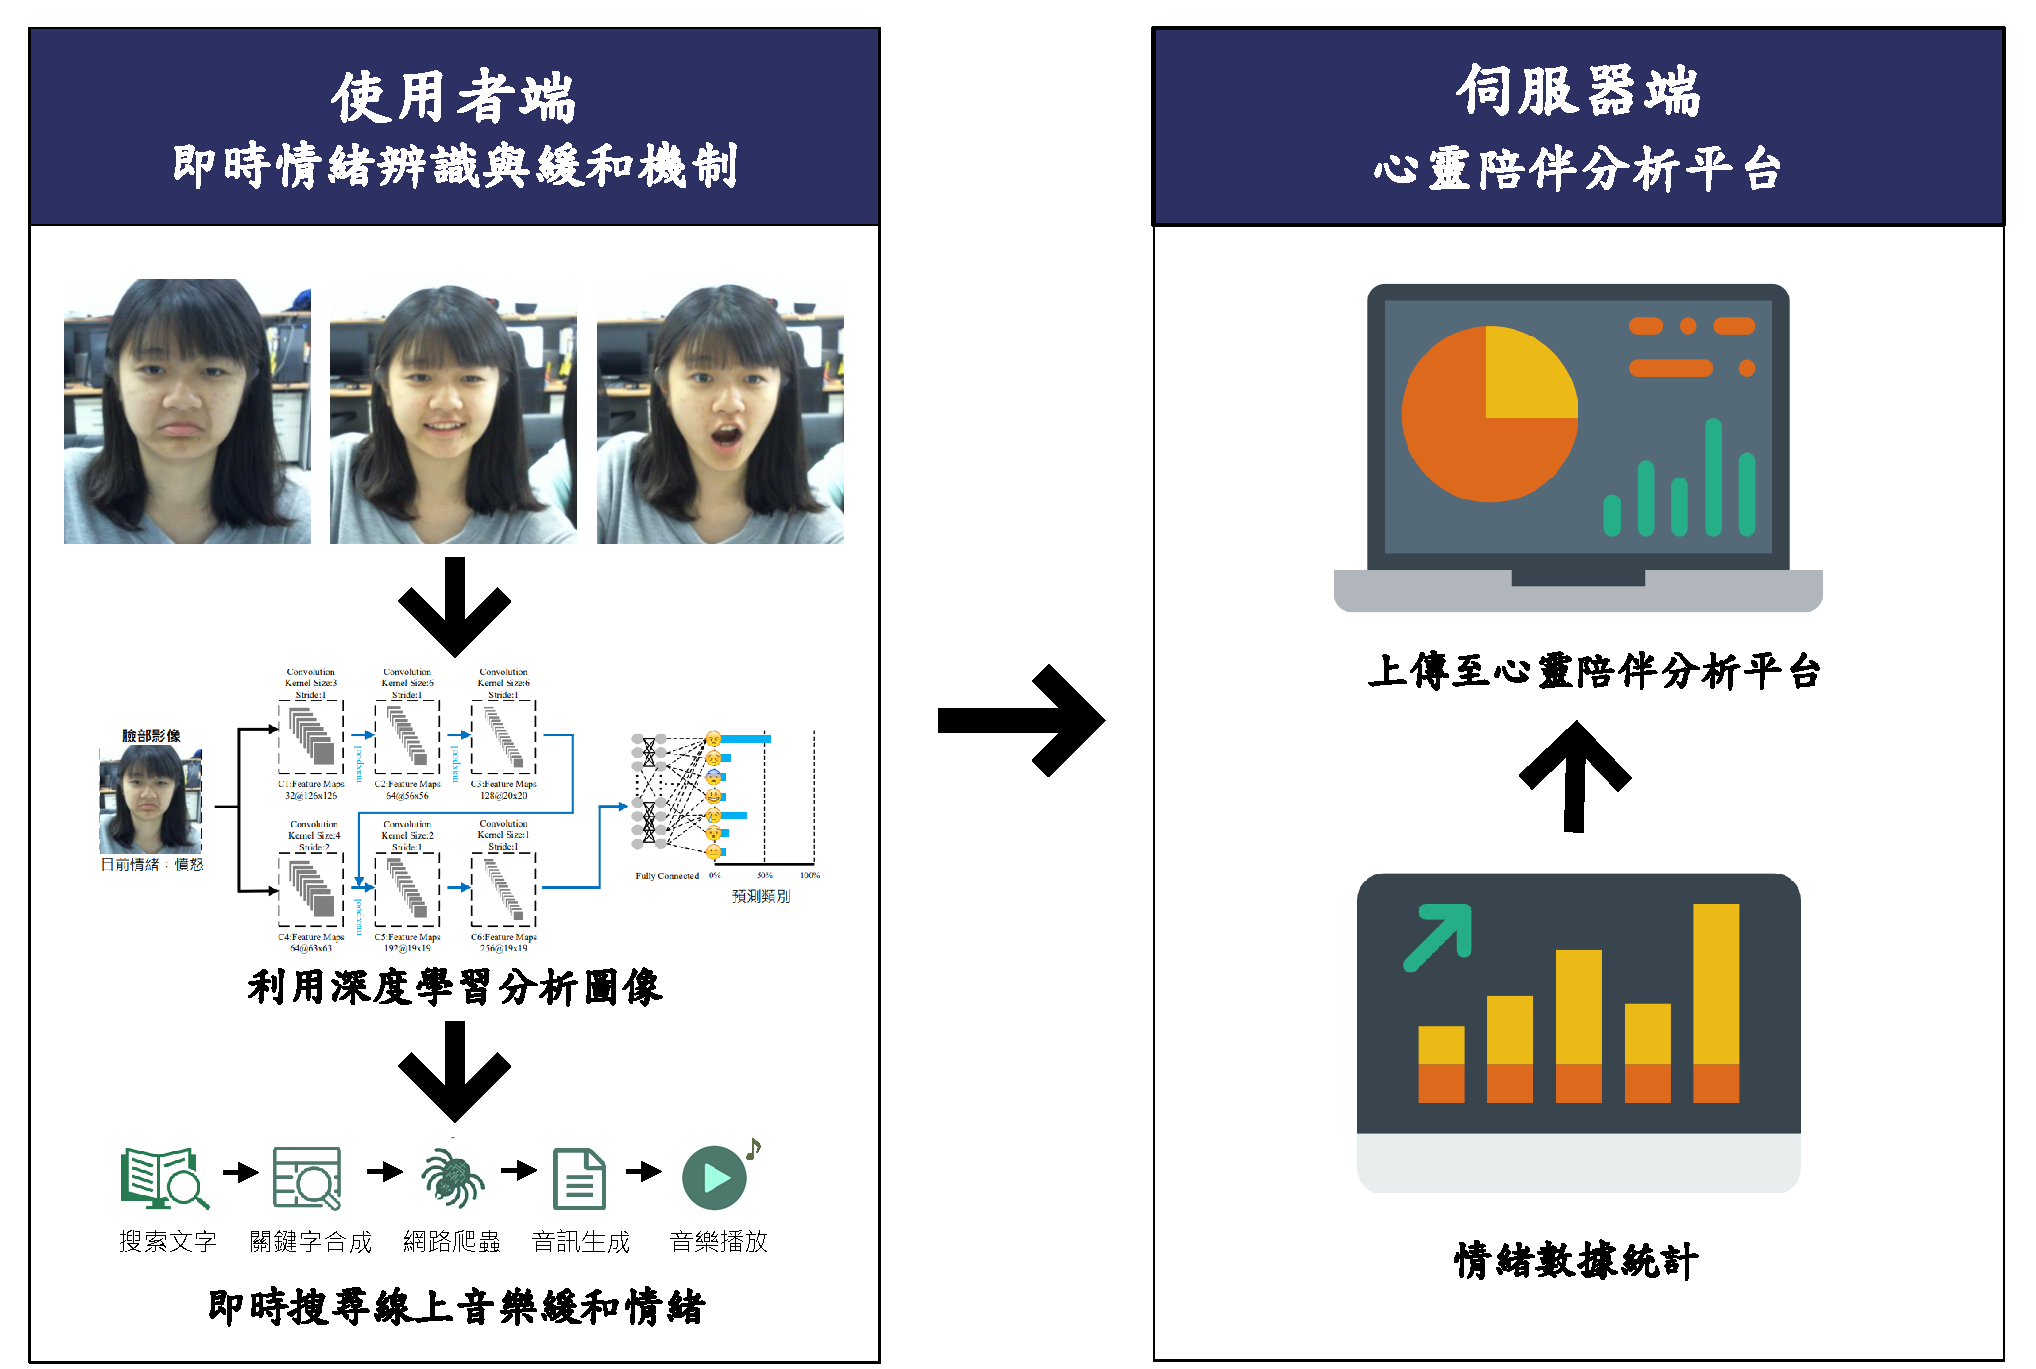
\includegraphics[width=9.4cm]{./Figures/UserAndServer.pdf}
\end{center}
\end{figure}

\end{frame}

\begin{frame}
\frametitle{作品介紹}
%使用者架構
\begin{itemize}
\item \Large使用者端 : 即時情緒辨識與緩和機制
\end{itemize}

\begin{figure}[!t]
\begin{center}
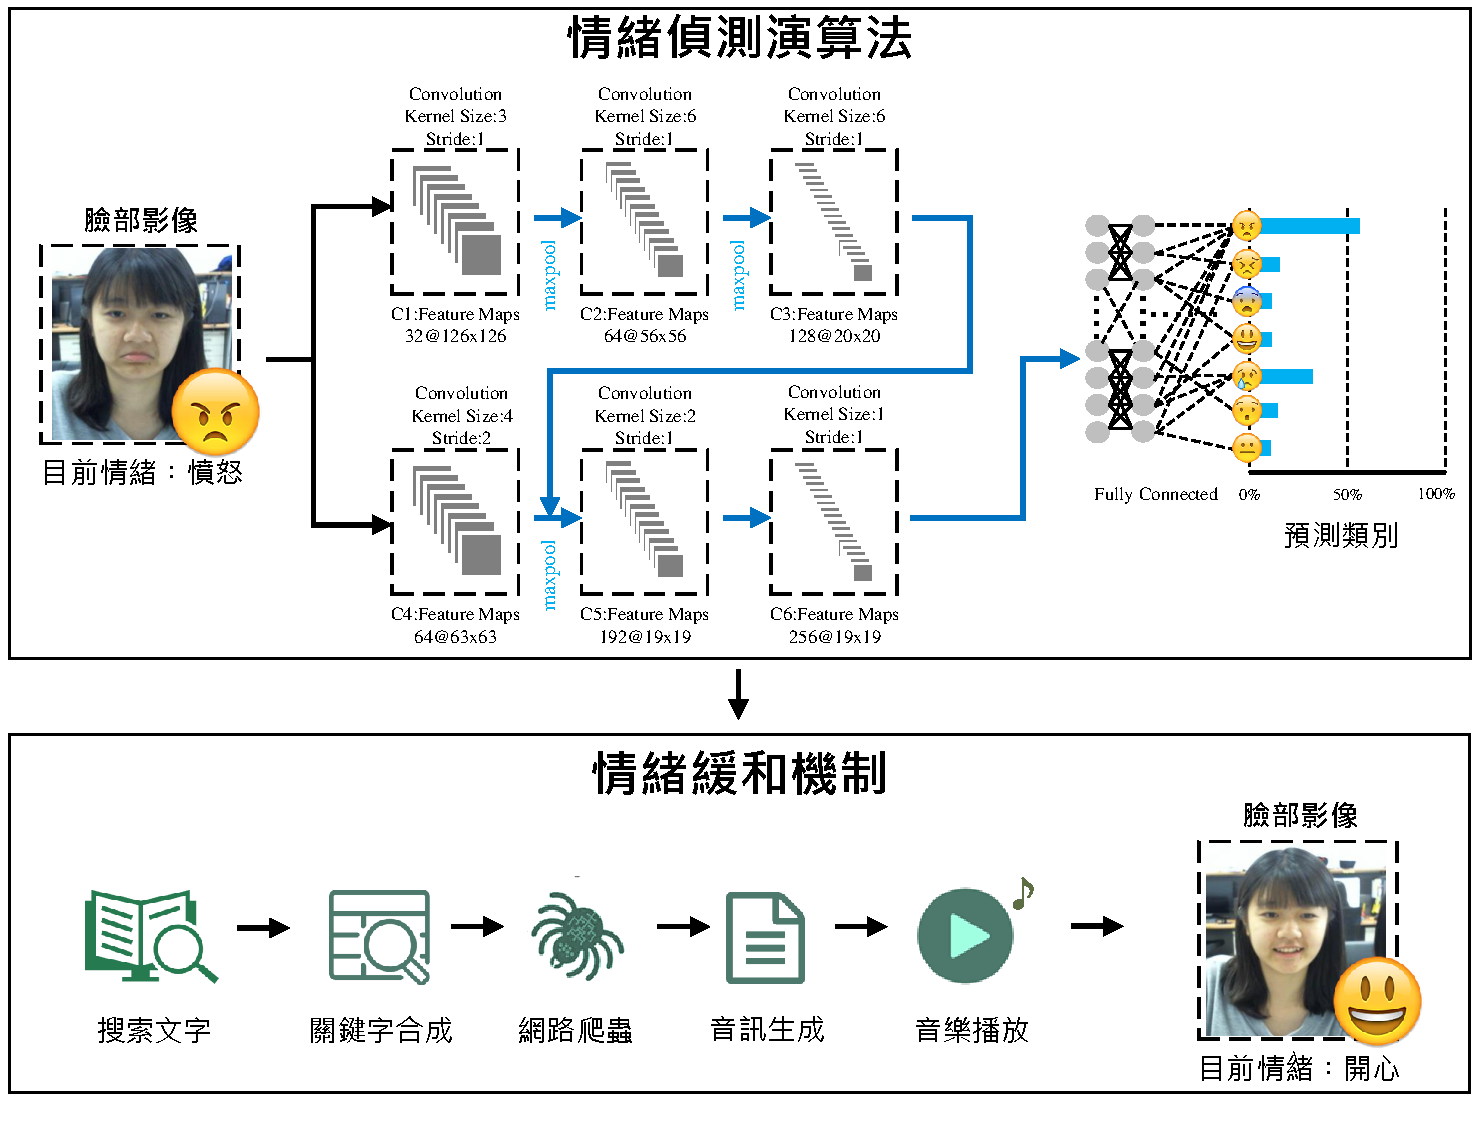
\includegraphics[width=9cm]{./Figures/framework_vertical.pdf}
\end{center}
\end{figure}

\end{frame}

\begin{frame}
\frametitle{作品介紹}
%偵測表情
\begin{figure}[t]
\begin{flushright}
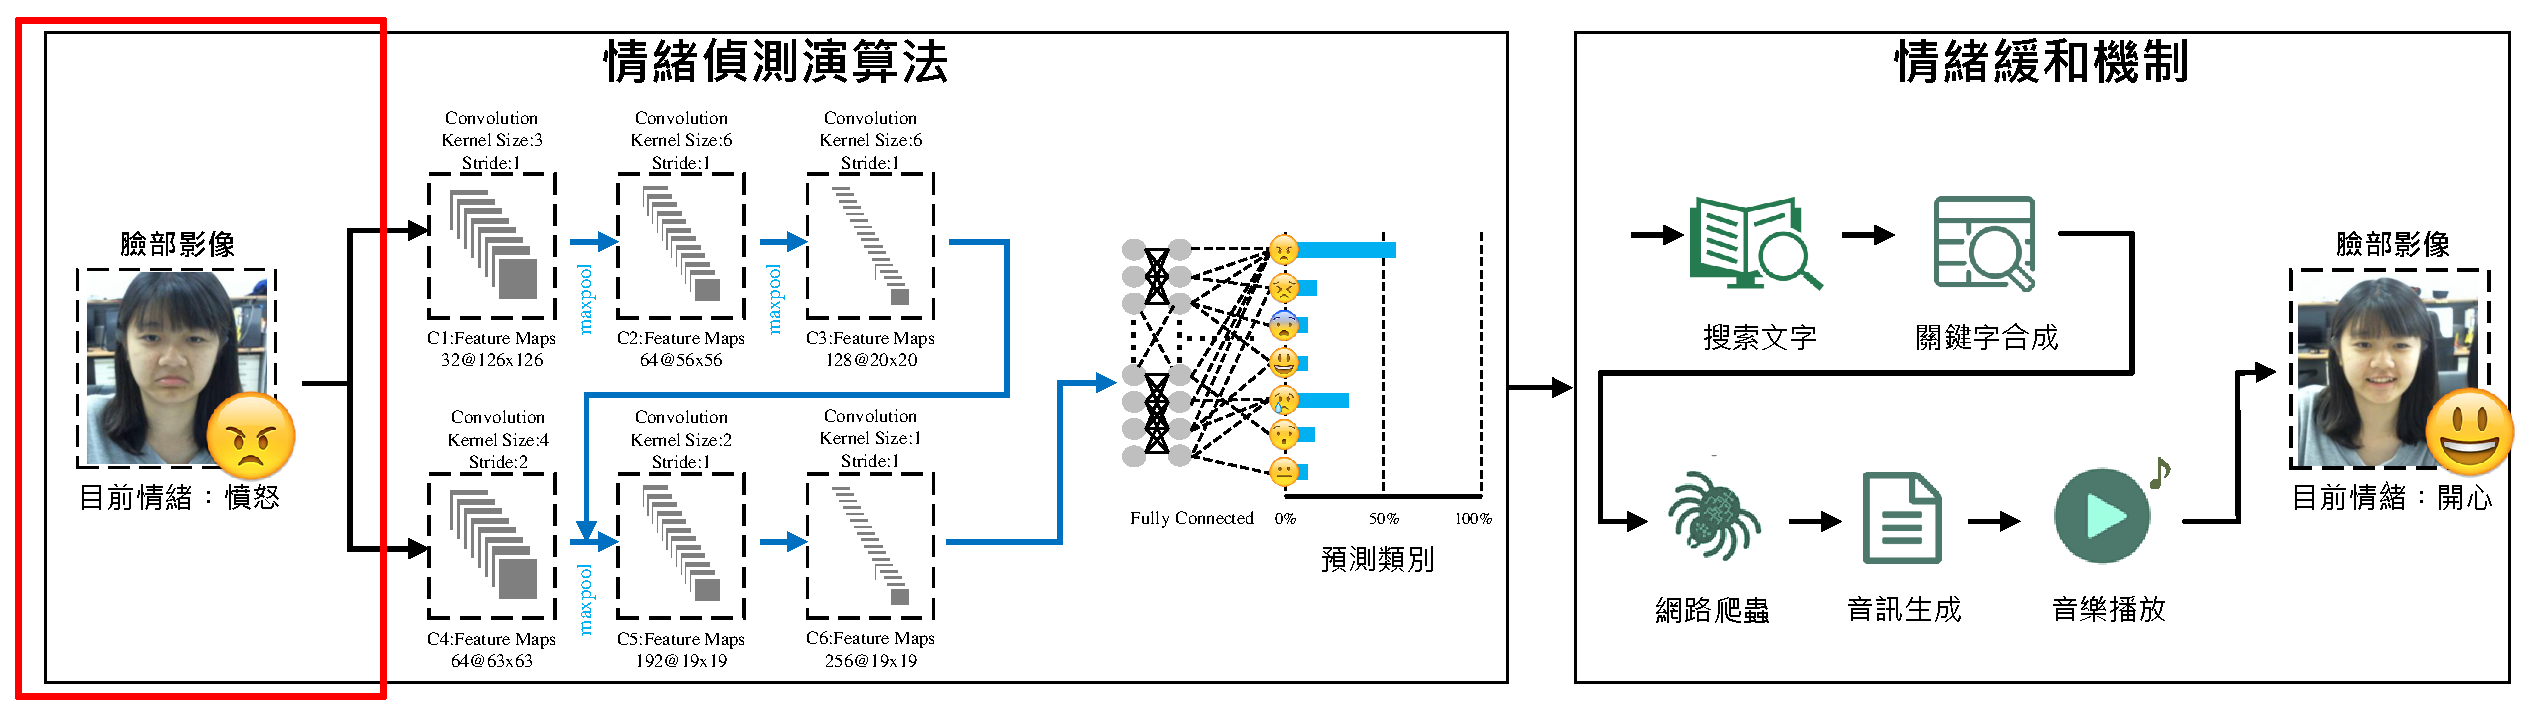
\includegraphics[width=5cm]{./Figures/framework1.pdf}
\end{flushright}
\end{figure}

\vspace{-9mm}
\begin{figure}[!t]
\begin{center}
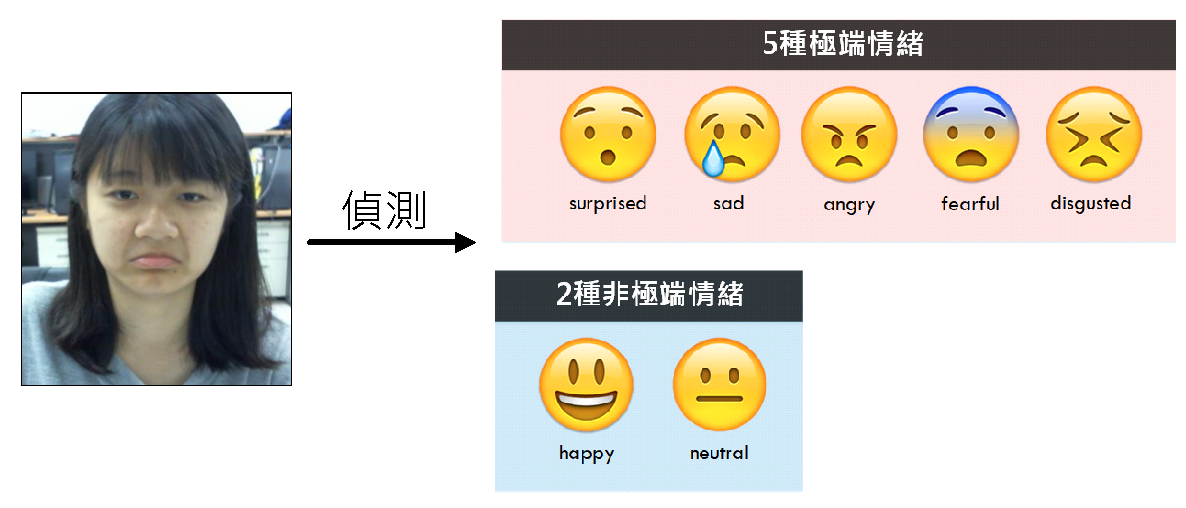
\includegraphics[width=12.3cm]{./Figures/Detect7Emotion.pdf}
\end{center}
\end{figure}

\end{frame}

\begin{frame}
\frametitle{作品介紹}
%卷積
\begin{figure}[t]
\begin{flushright}
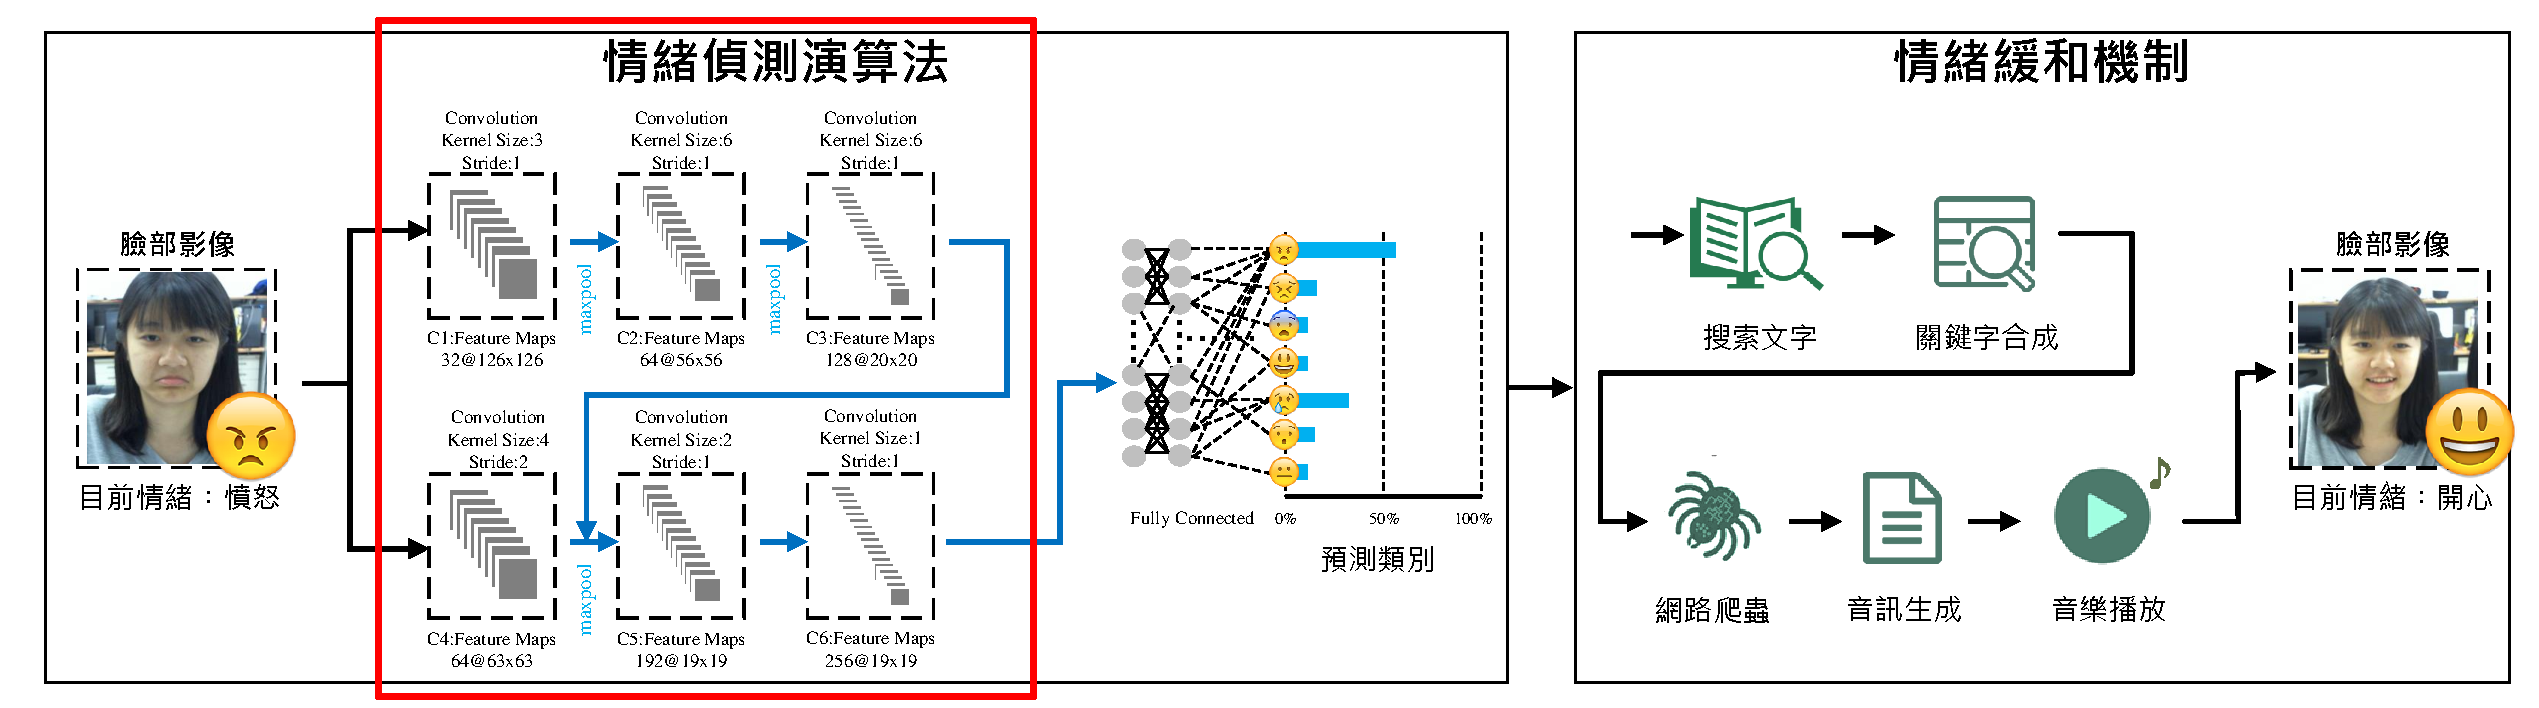
\includegraphics[width=5cm]{./Figures/framework2.pdf}
\end{flushright}
\end{figure}

\vspace{-5mm}
\begin{figure}[!t]
\begin{center}
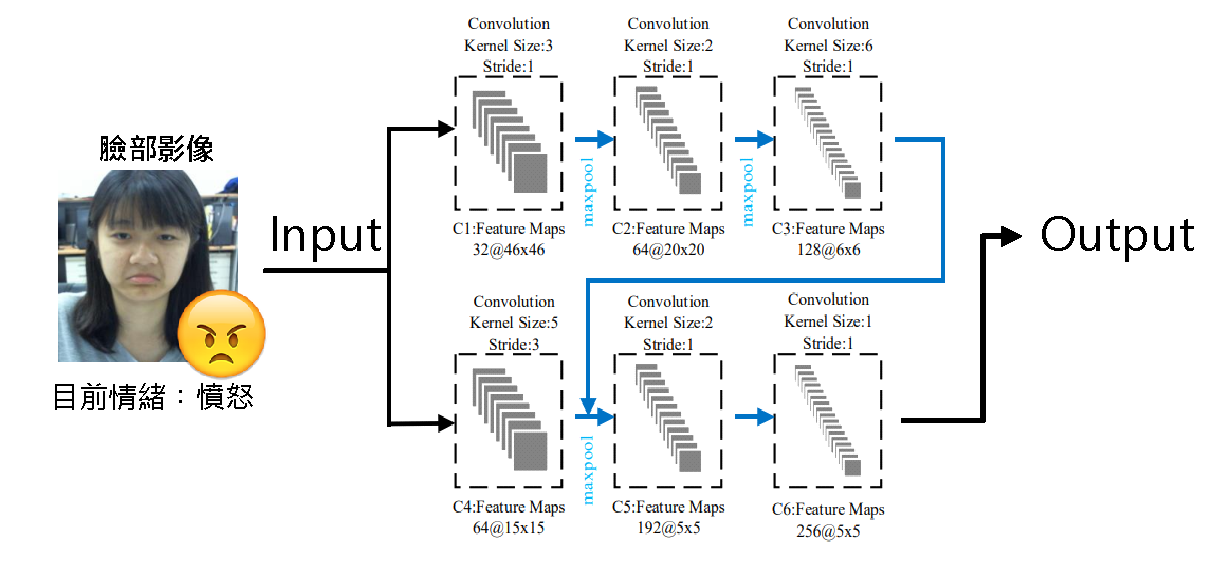
\includegraphics[width=12.3cm]{./Figures/FrameworkFirst.pdf}
\end{center}
\end{figure}

\end{frame}

\begin{frame}
\frametitle{作品介紹}
%表情進資料庫
\begin{figure}[t]
\begin{flushright}
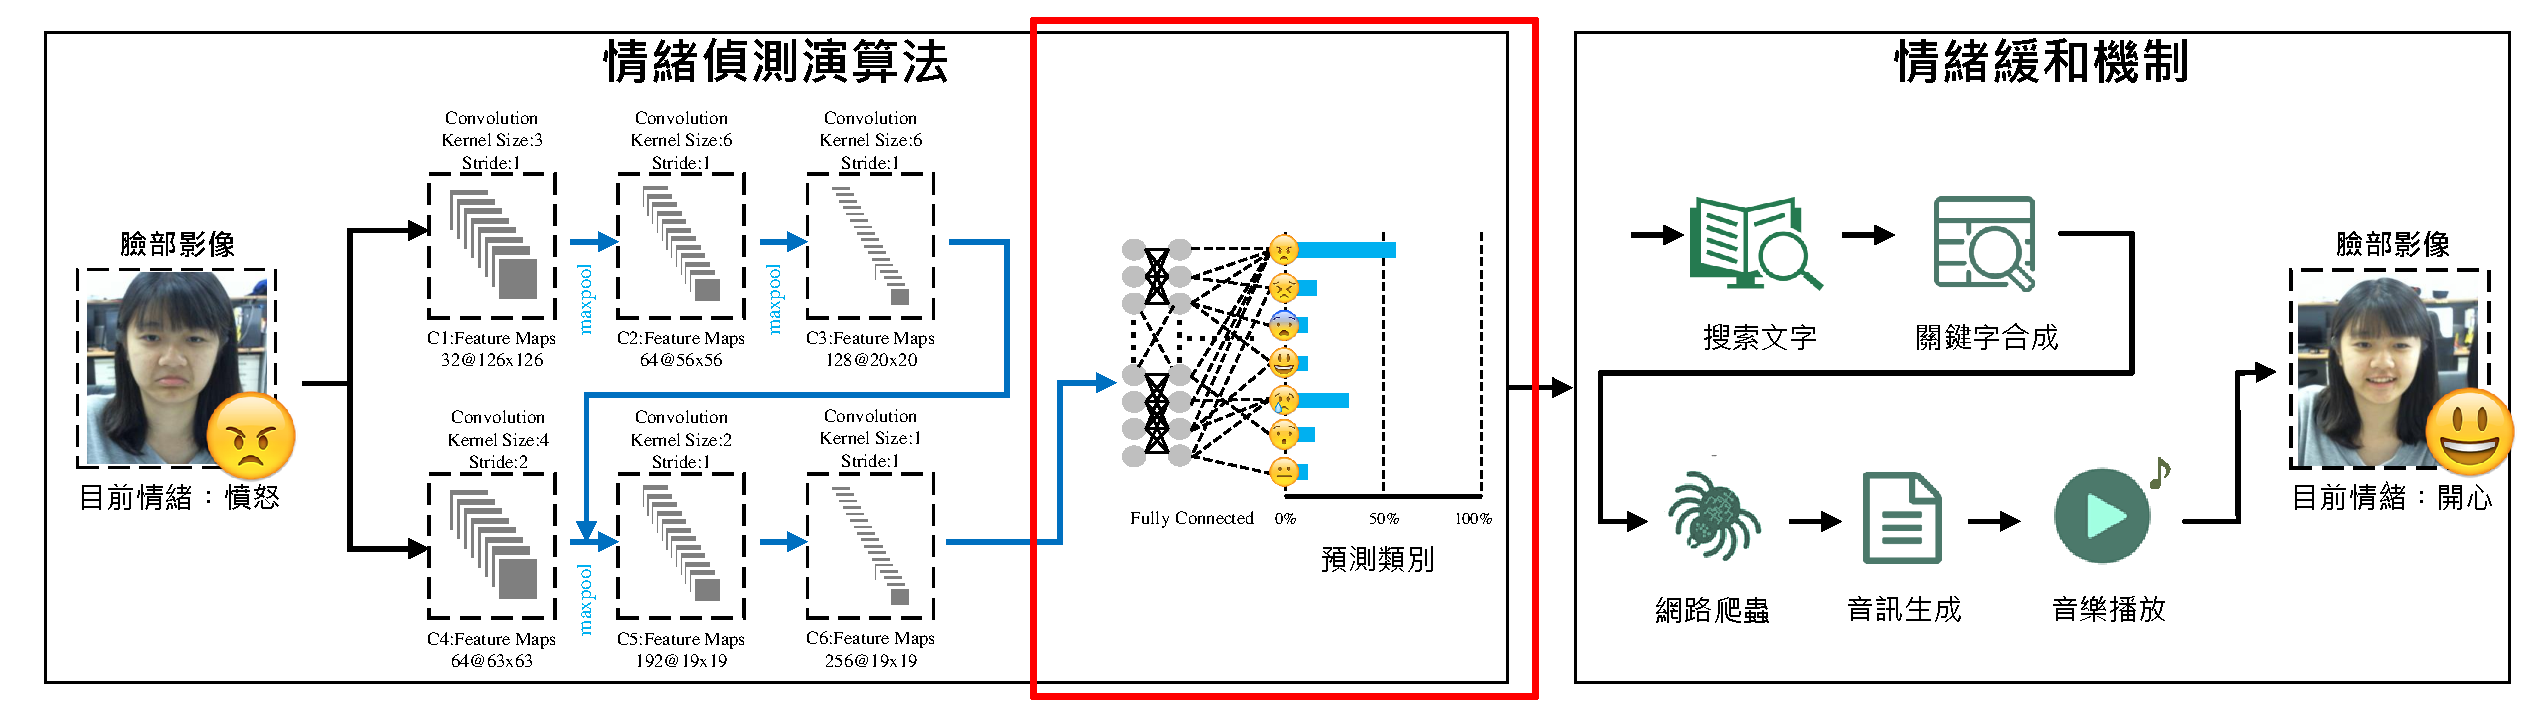
\includegraphics[width=5cm]{./Figures/framework3.pdf}
\end{flushright}
\end{figure}

\vspace{-5mm}

\begin{itemize}
\item \Large將表情放入資料庫
\end{itemize}

\vspace{5mm}
\begin{figure}[!t]
\begin{center}
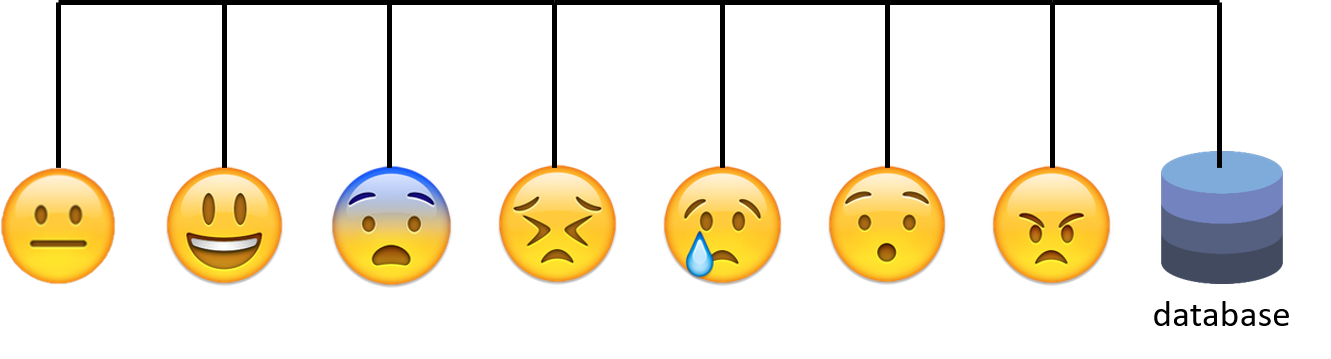
\includegraphics[width=12.3cm]{./Figures/501.png}
\end{center}
\end{figure}

\end{frame}

\begin{frame}
\frametitle{作品介紹}
%voting1
\begin{figure}[t]
\begin{flushright}
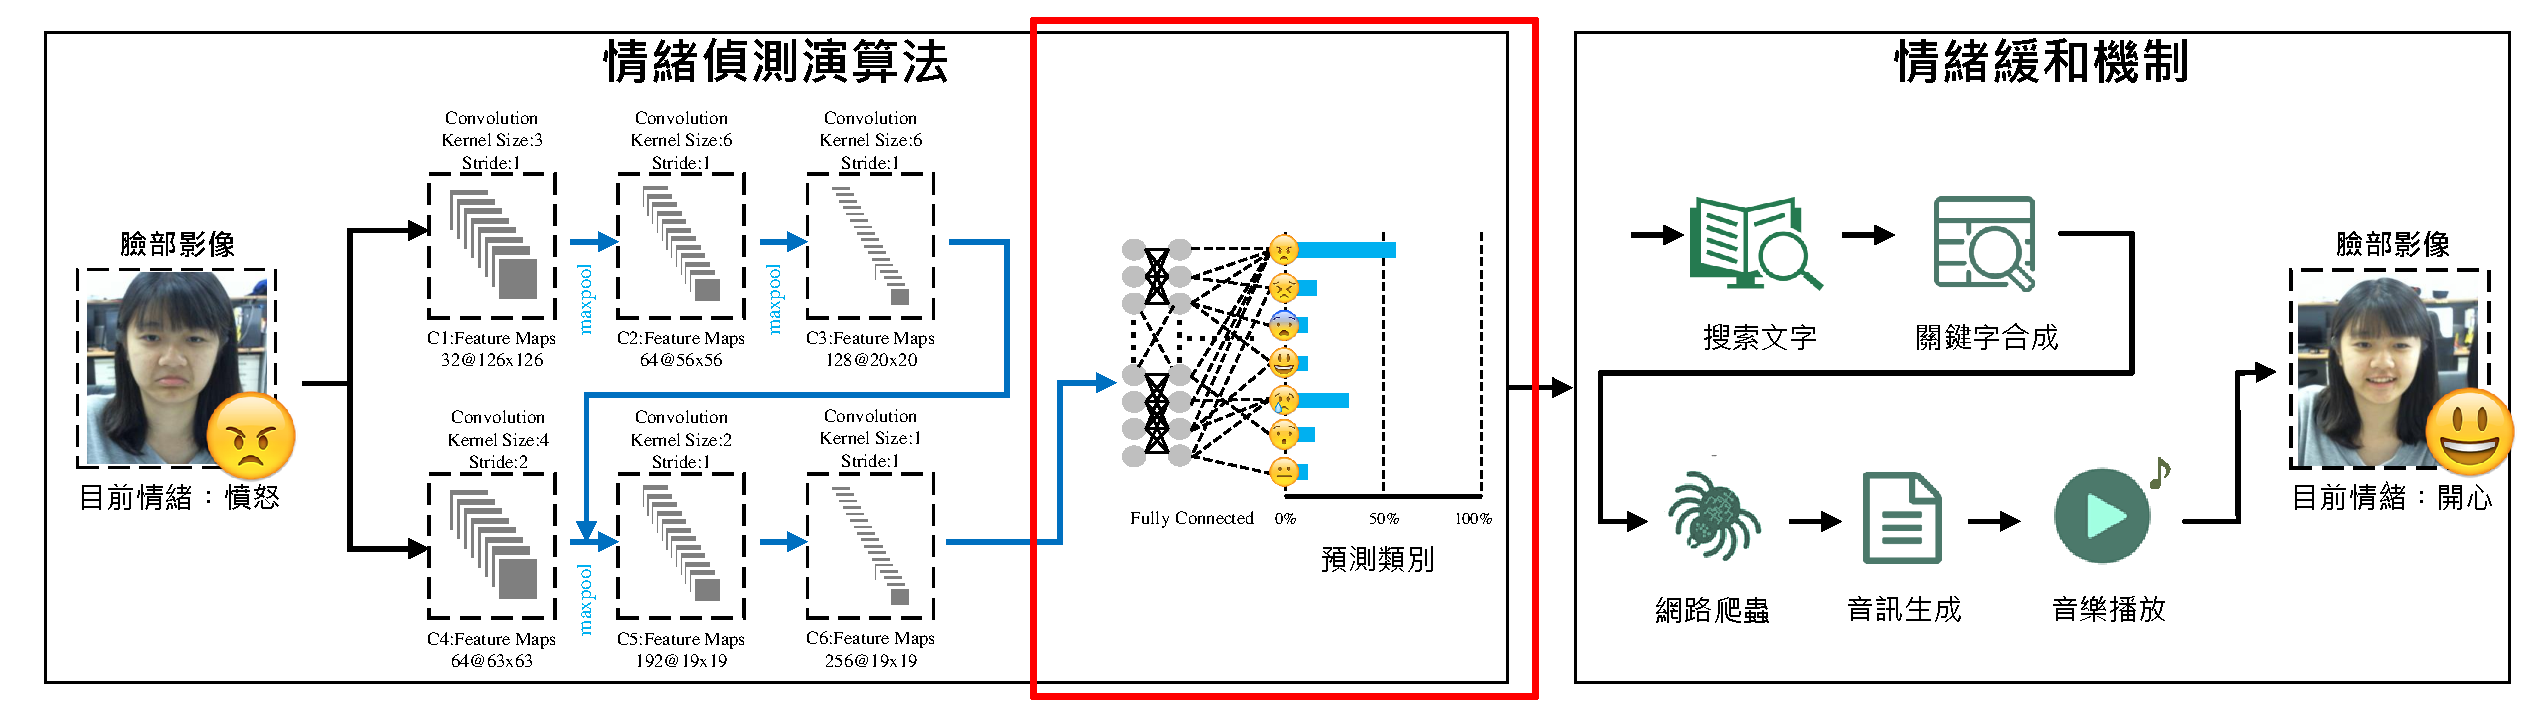
\includegraphics[width=5cm]{./Figures/framework3.pdf}
\end{flushright}
\end{figure}

\vspace{-5mm}
\begin{figure}[!t]
\begin{center}
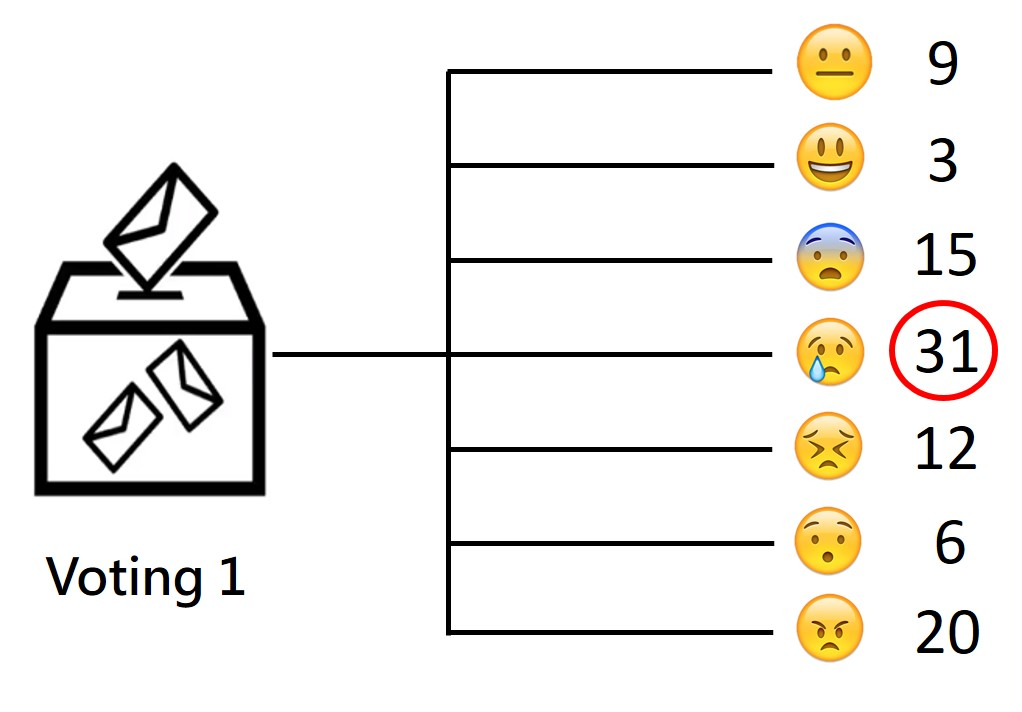
\includegraphics[width=9cm]{./Figures/502.jpg}
\end{center}
\end{figure}

\end{frame}

\begin{frame}
\frametitle{作品介紹}
%voting2
\begin{figure}[t]
\begin{flushright}
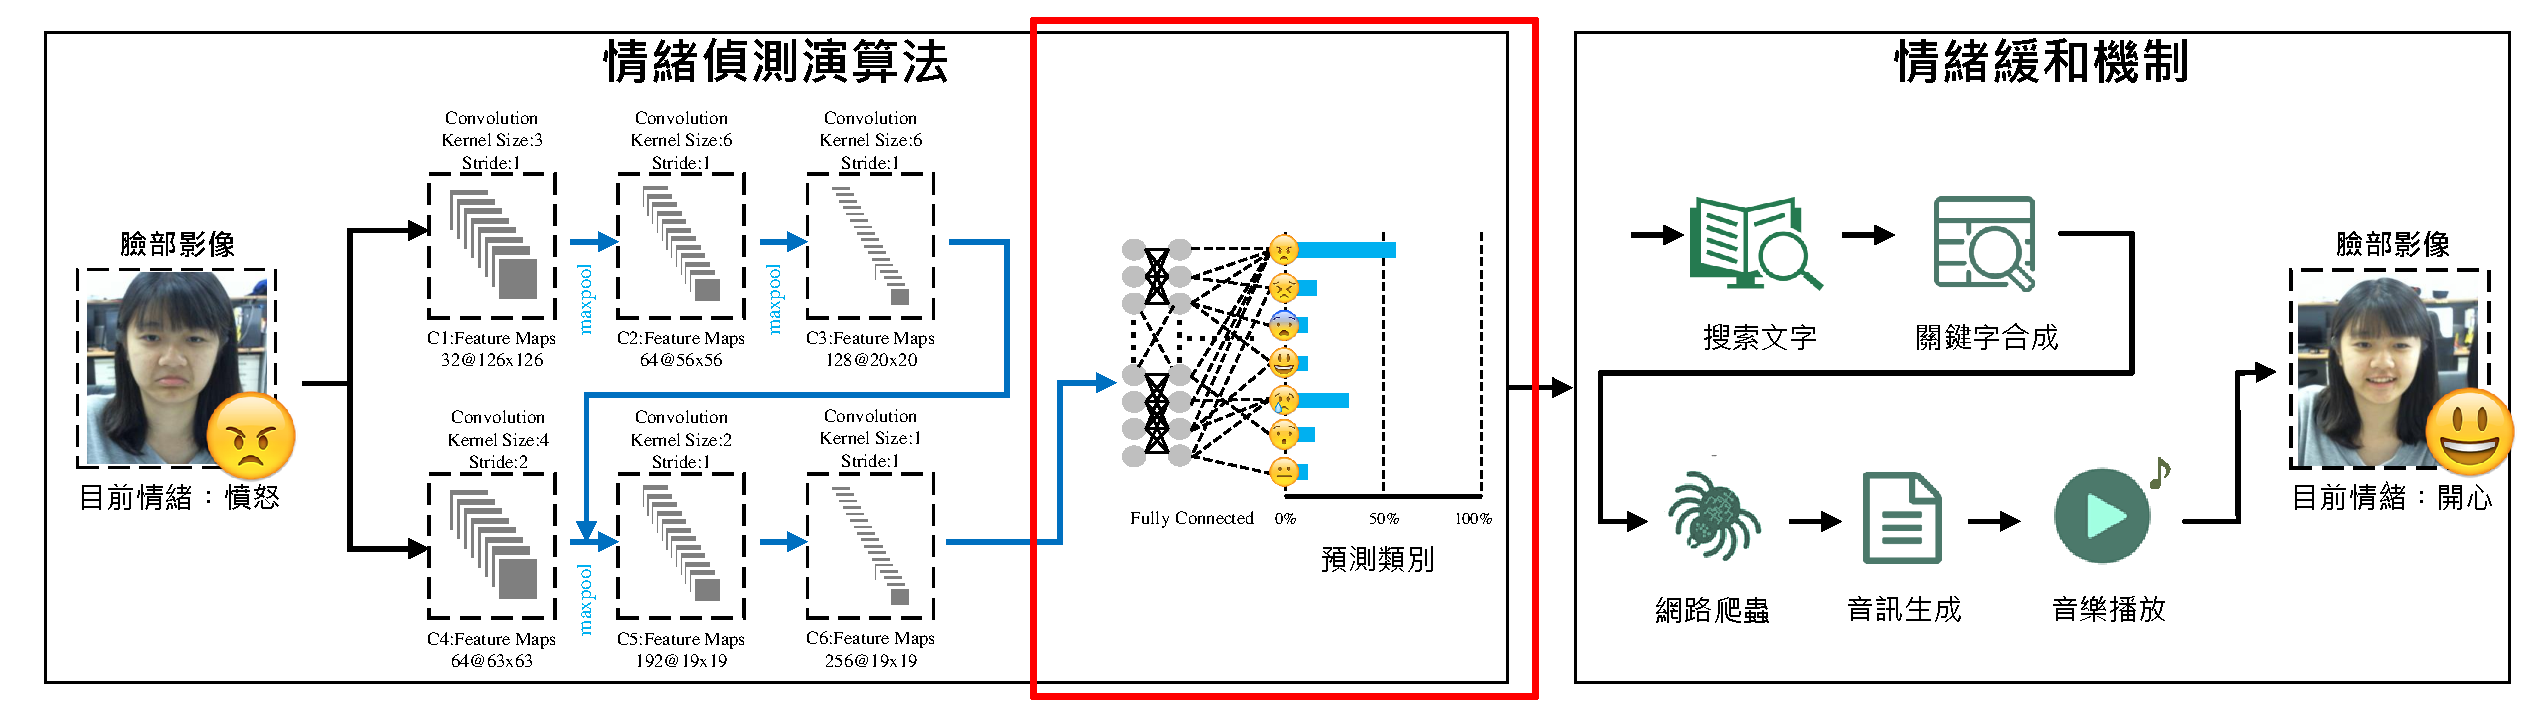
\includegraphics[width=5cm]{./Figures/framework3.pdf}
\end{flushright}
\end{figure}

\vspace{-5mm}
\begin{figure}[!t]
\begin{center}
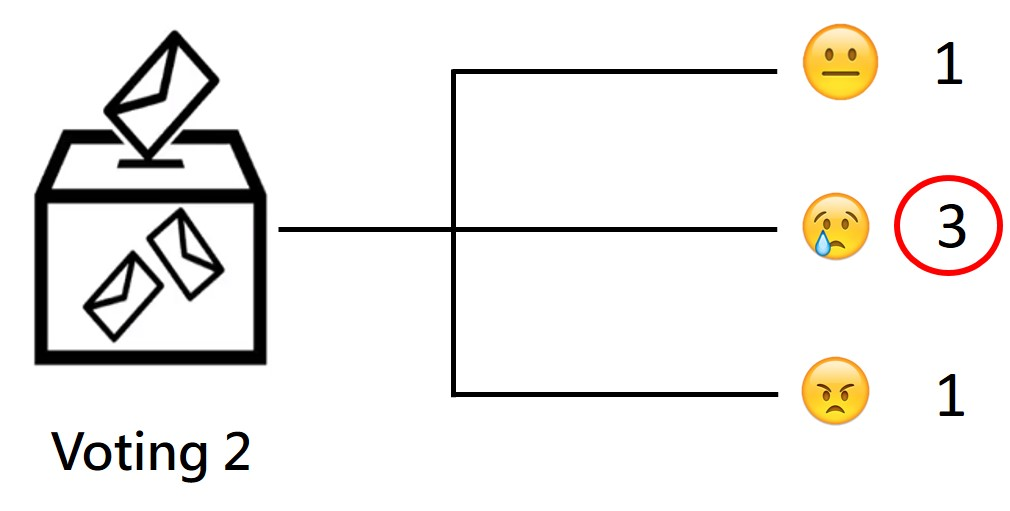
\includegraphics[width=9cm]{./Figures/503.jpg}
\end{center}
\end{figure}

\end{frame}

\begin{frame}
\frametitle{作品介紹}
%偵測結果

\begin{figure}[t]
\begin{flushright}
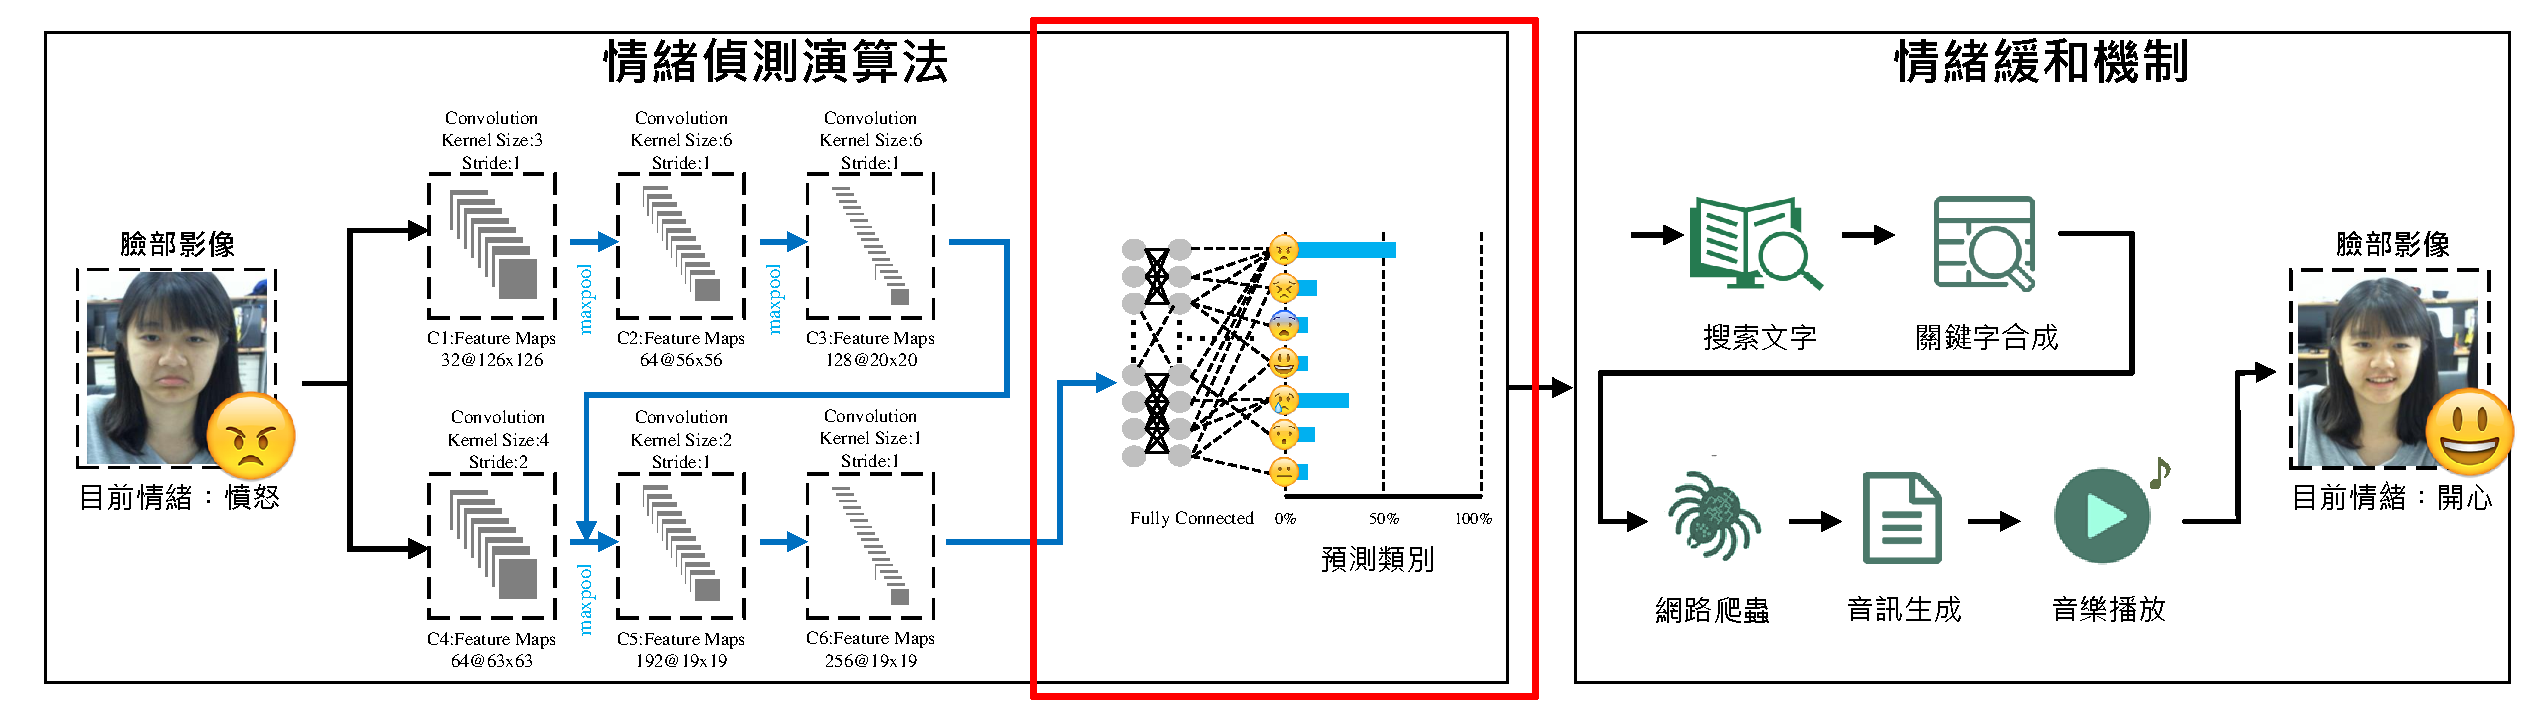
\includegraphics[width=5cm]{./Figures/framework3.pdf}
\end{flushright}
\end{figure}

\vspace{-5mm}

\begin{itemize}
\item \Large偵測結果
\end{itemize}


\begin{figure}[!t]
\begin{center}
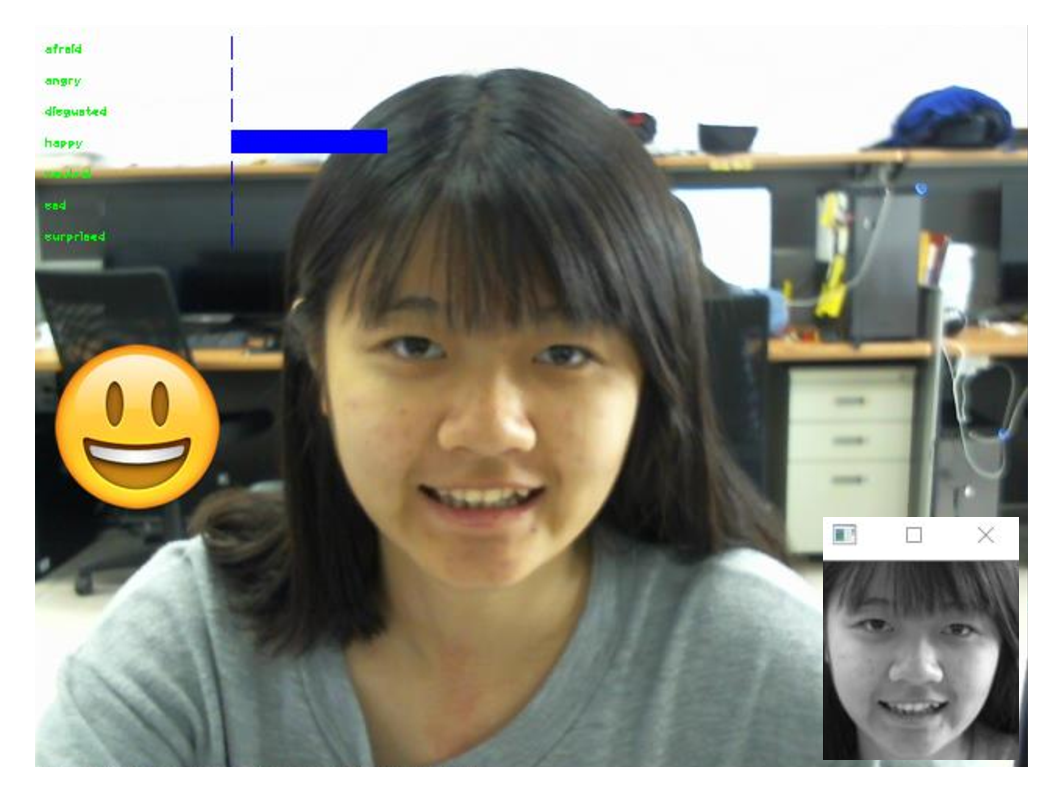
\includegraphics[width=8cm]{./Figures/DetectResult.pdf}
\end{center}
\end{figure}
\end{frame}

\begin{frame}
\frametitle{作品介紹}
%情緒機制

\vspace{-15mm}
\begin{figure}[t]
\begin{flushright}
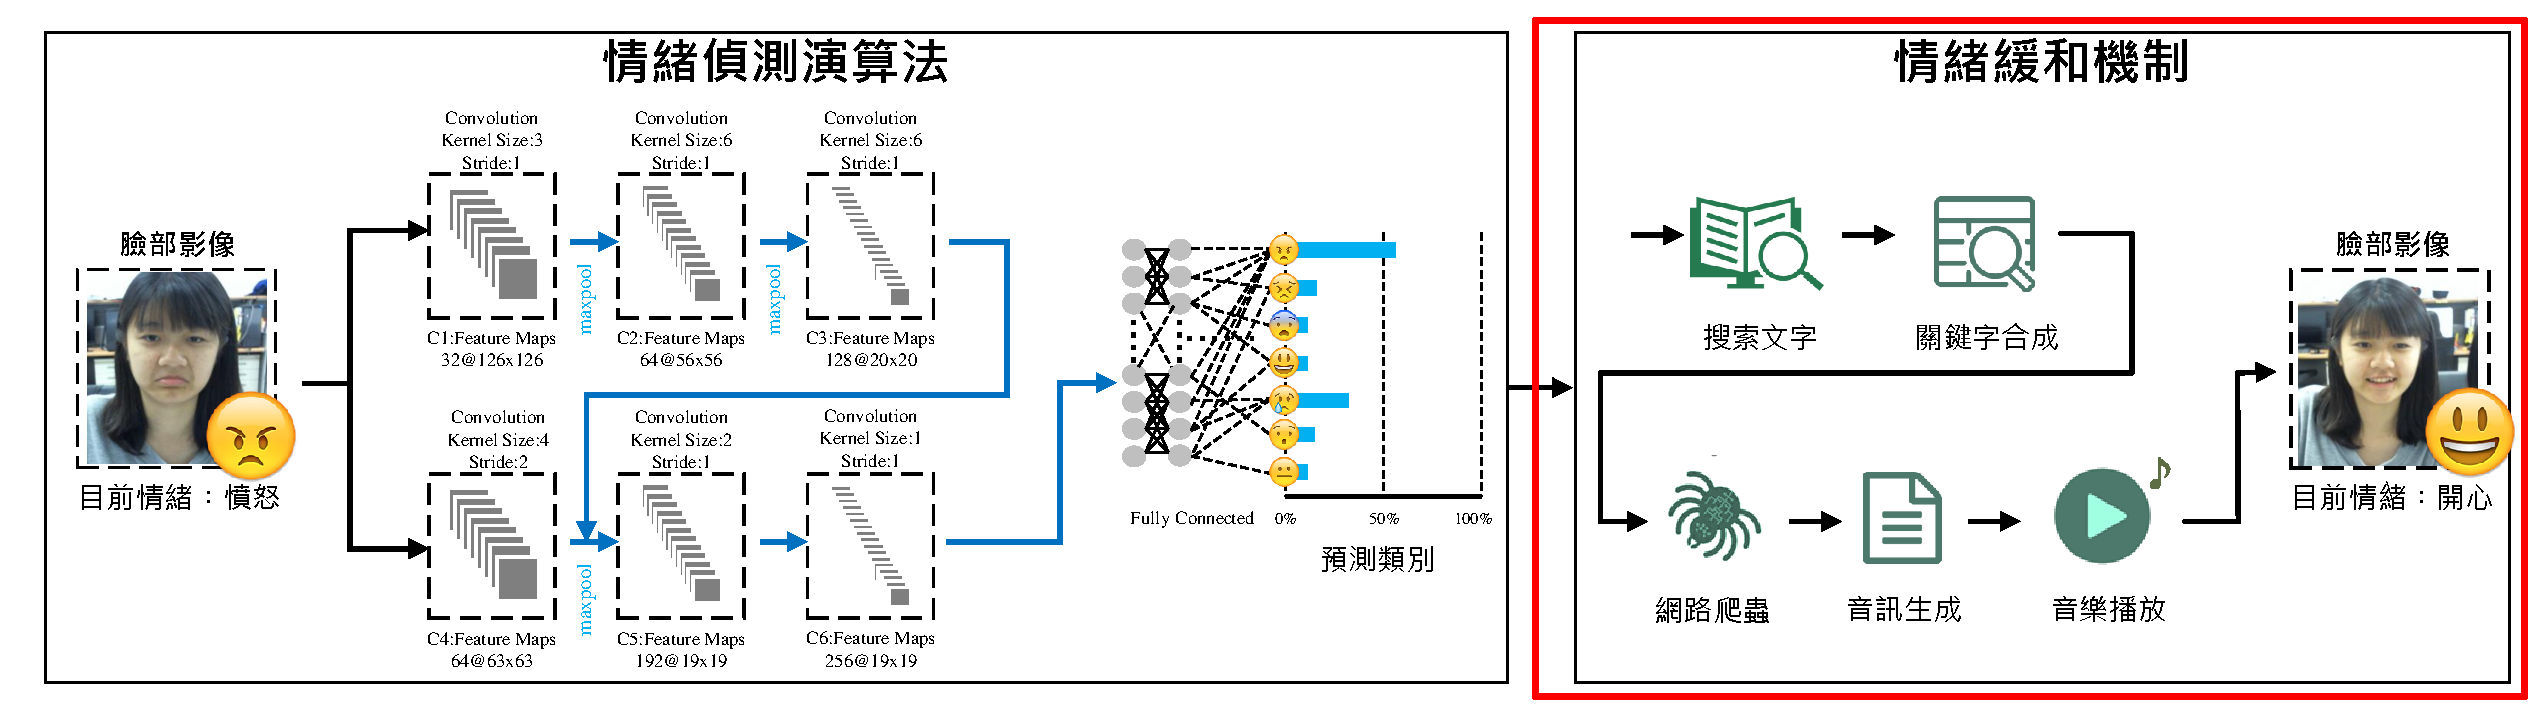
\includegraphics[width=5cm]{./Figures/framework9.pdf}
\end{flushright}
\end{figure}

\vspace{-5mm}

\begin{itemize}
\item \Large情緒緩和機制
\end{itemize}

\begin{figure}[!t]
\begin{center}
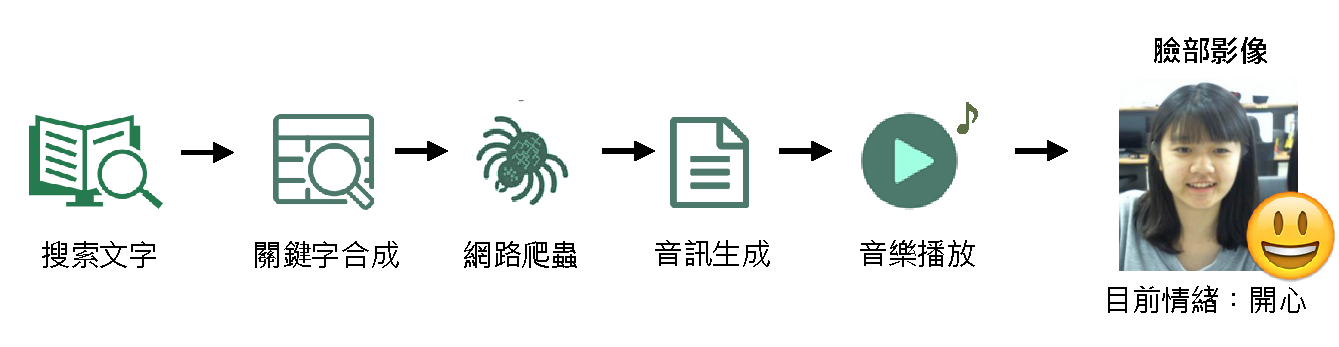
\includegraphics[width=12cm]{./Figures/FrameworkSecond.pdf}
\end{center}
\end{figure}
\end{frame}

\begin{frame}
\frametitle{作品介紹}
%緩和文字

\vspace{-5mm}
\begin{figure}[t]
\begin{flushright}
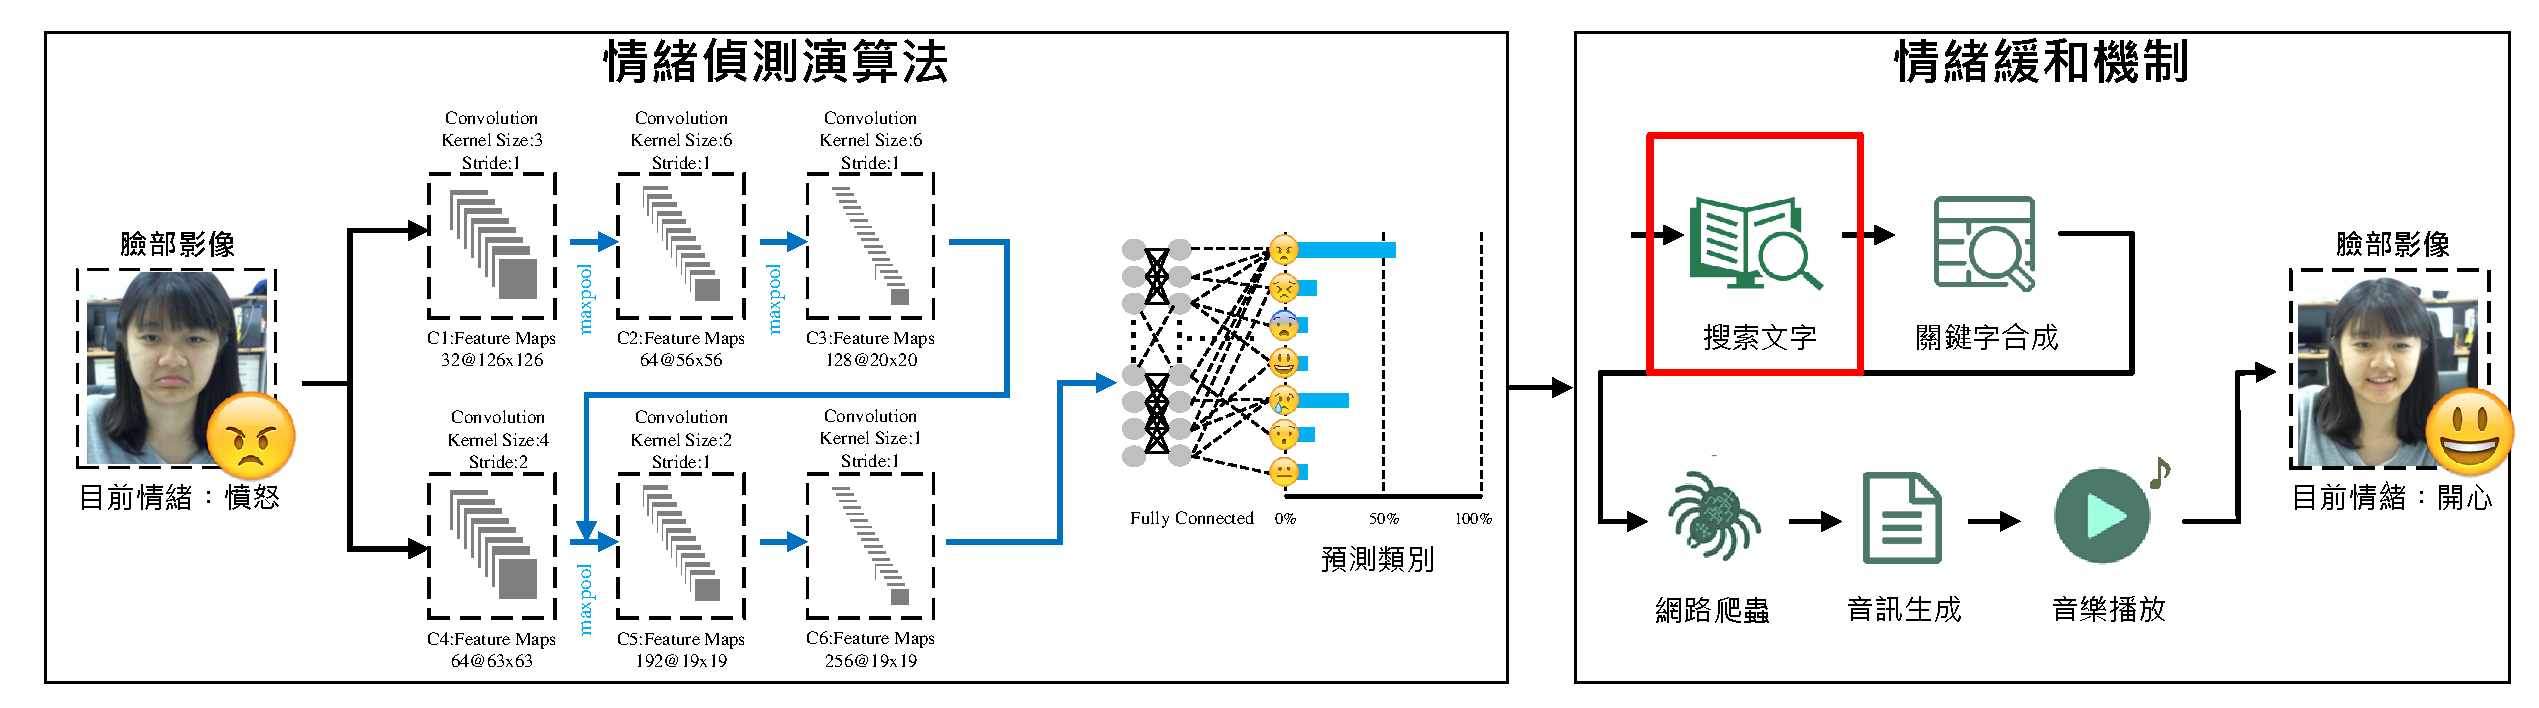
\includegraphics[width=5cm]{./Figures/framework4.pdf}
\end{flushright}
\end{figure}

\vspace{-5mm}

\begin{itemize}
\item \Large緩和情緒文字
\end{itemize}

\begin{figure}[!t]
\begin{center}
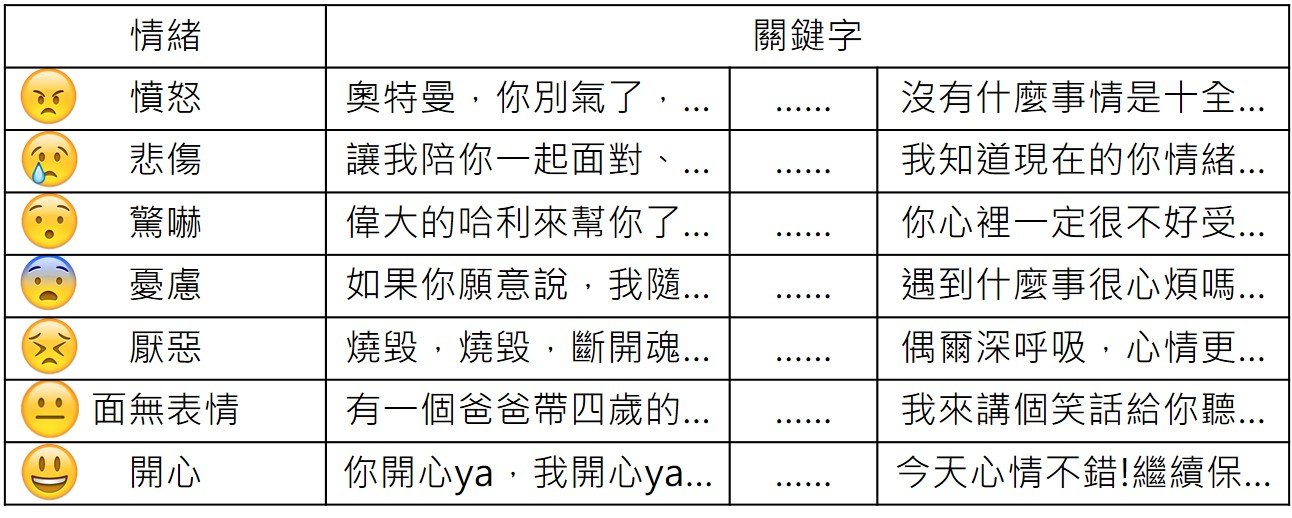
\includegraphics[width=12cm]{./Figures/505.jpg}
\end{center}
\end{figure}
\end{frame}

\begin{frame}
\frametitle{作品介紹}
%關鍵字

\vspace{-5mm}
\begin{figure}[t]
\begin{flushright}
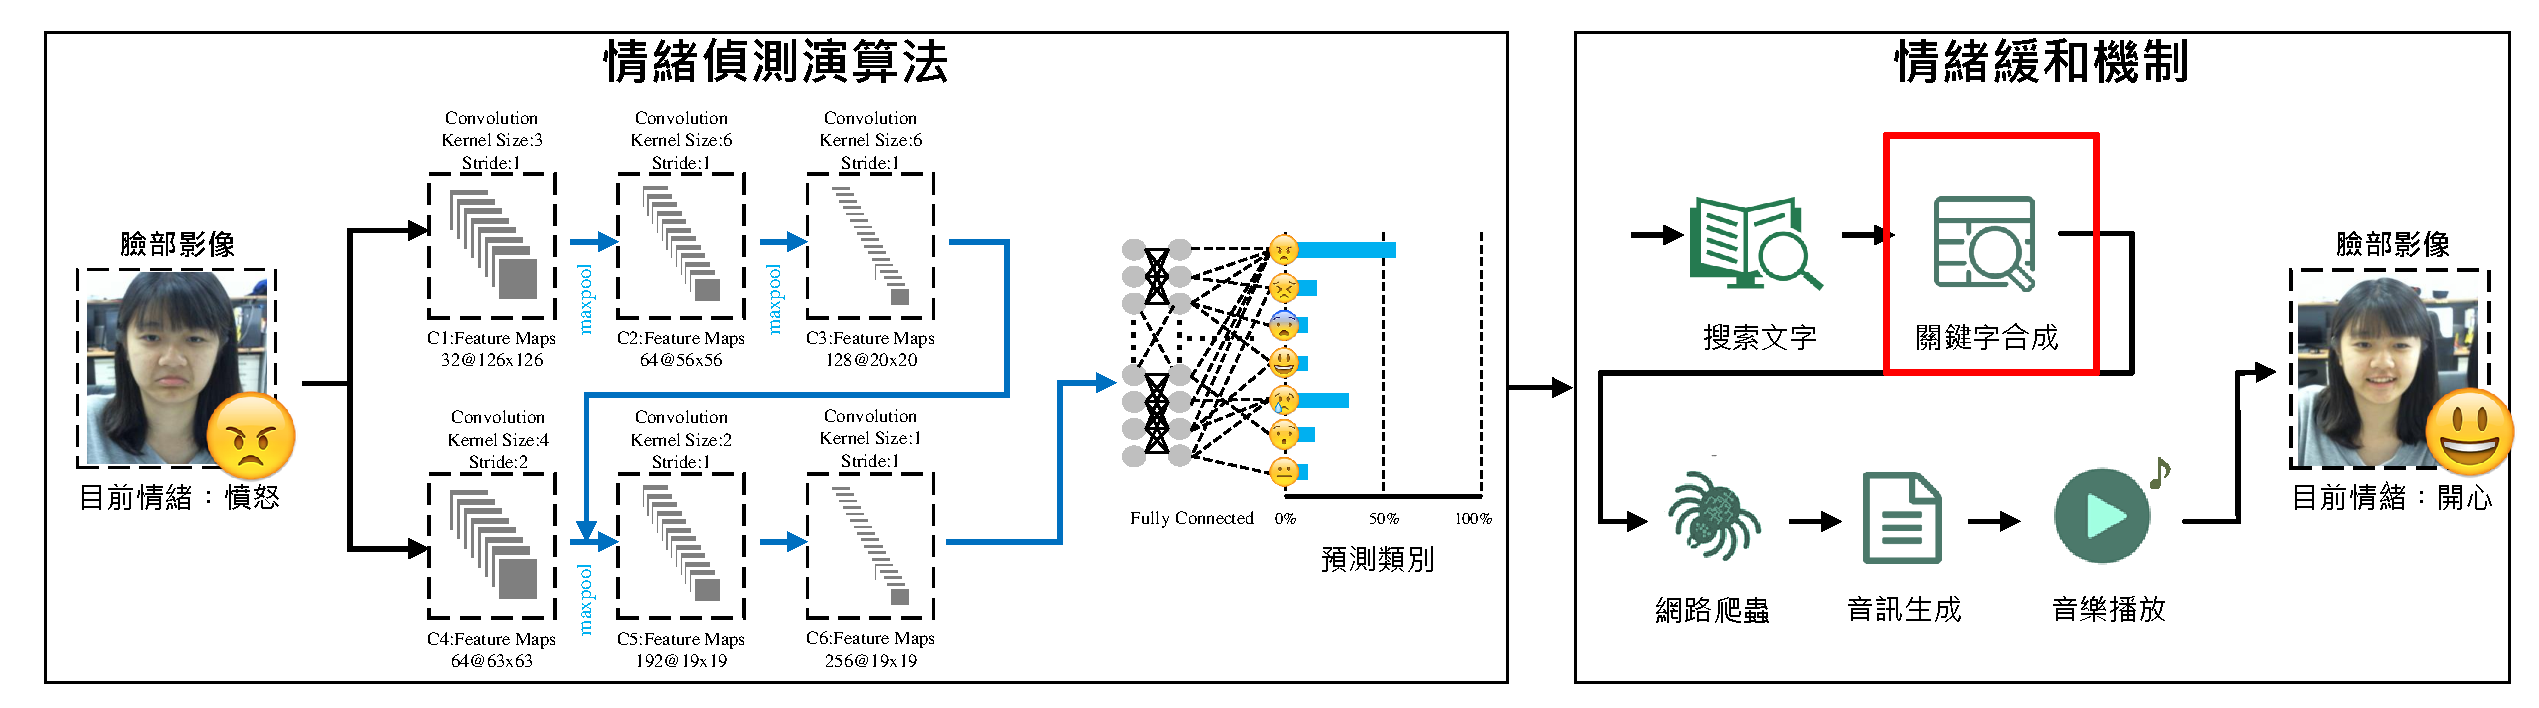
\includegraphics[width=5cm]{./Figures/framework5.pdf}
\end{flushright}
\end{figure}

\vspace{-5mm}

\begin{itemize}
\item \Large關鍵字合成表
\end{itemize}

\begin{figure}[!t]
\begin{center}
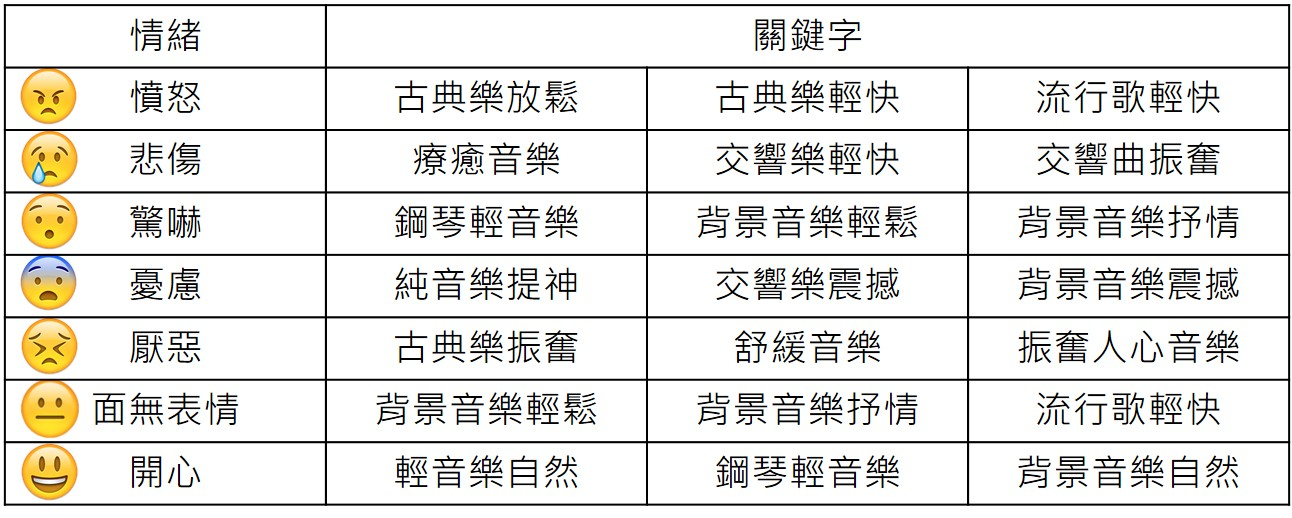
\includegraphics[width=12cm]{./Figures/504.jpg}
\end{center}
\end{figure}
\end{frame}

\begin{frame}
\frametitle{作品介紹}
%爬蟲

\vspace{-5mm}
\begin{figure}[t]
\begin{flushright}
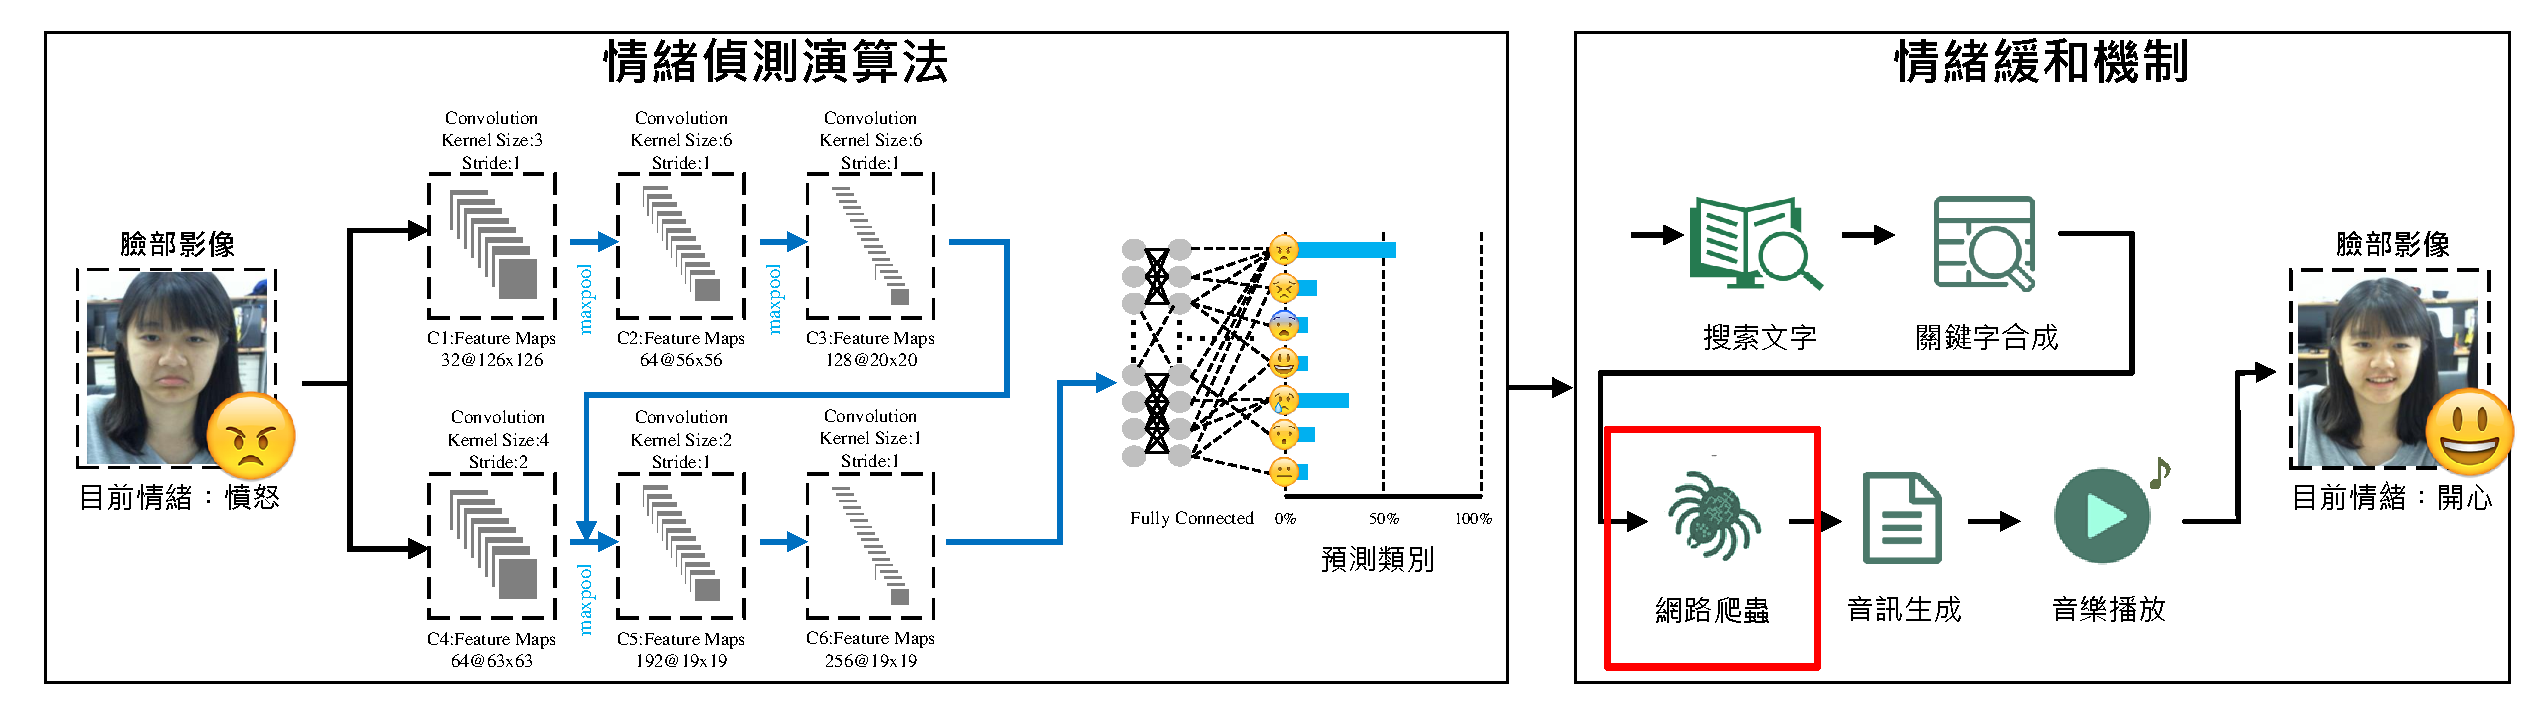
\includegraphics[width=5cm]{./Figures/framework6.pdf}
\end{flushright}
\end{figure}

\vspace{-5mm}

\begin{itemize}
\item \Large網路爬蟲
\end{itemize}

\begin{figure}[!t]
\begin{center}

\includegraphics[width=12cm]{./Figures/506.jpg}
\end{center}
\end{figure}
\end{frame}

\begin{frame}
\frametitle{作品介紹}
%音訊

\vspace{-5mm}
\begin{figure}[t]
\begin{flushright}
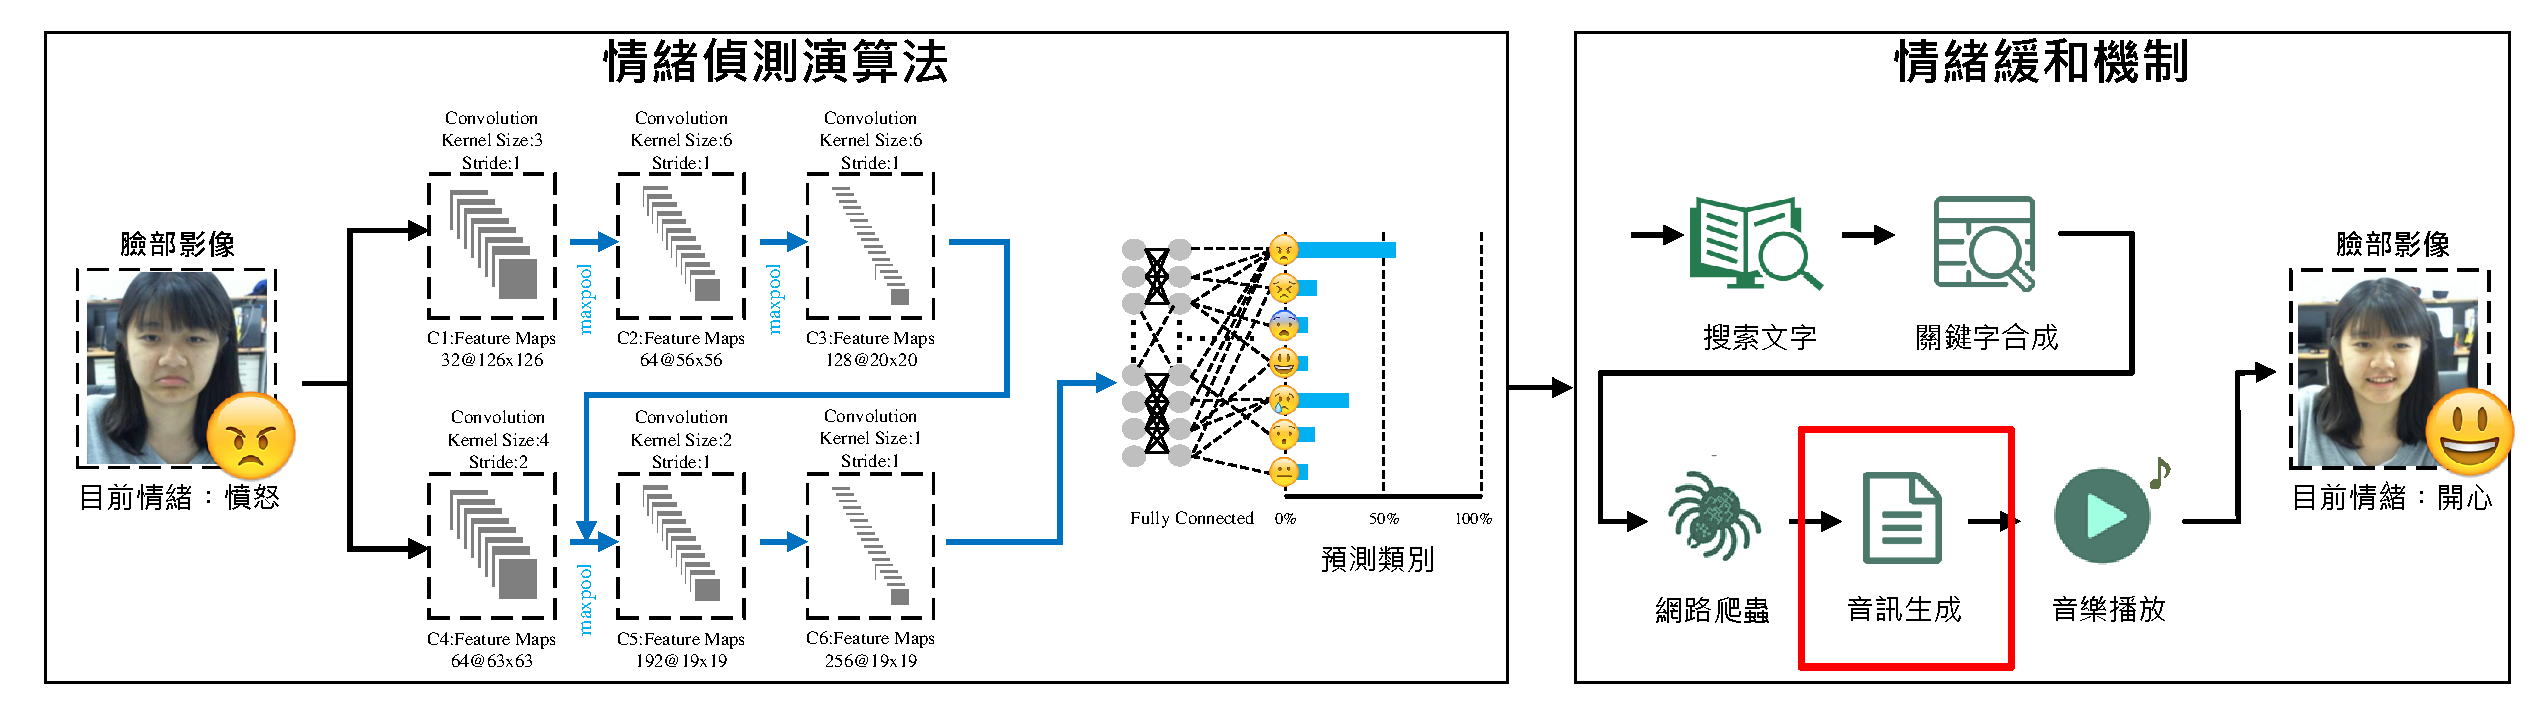
\includegraphics[width=5cm]{./Figures/framework7.pdf}
\end{flushright}
\end{figure}

\vspace{-5mm}

\begin{itemize}
\item \Large音訊生成
\end{itemize}

\begin{figure}[!t]
\begin{center}
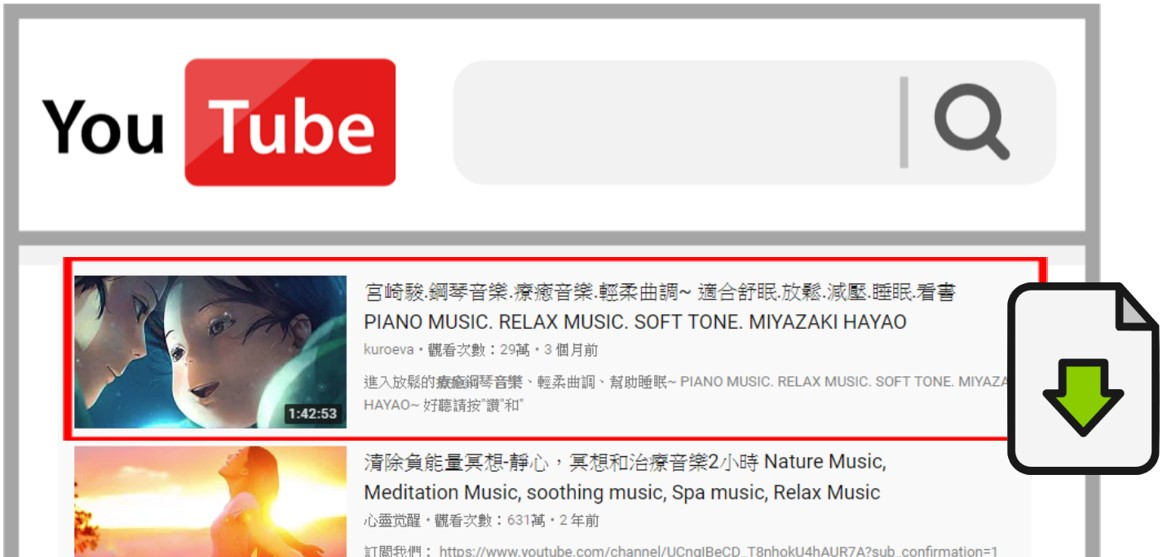
\includegraphics[width=10cm]{./Figures/507.jpg}
\end{center}
\end{figure}
\end{frame}

\begin{frame}
\frametitle{作品介紹}
%結果

\vspace{-3mm}
\begin{figure}[t]
\begin{flushright}
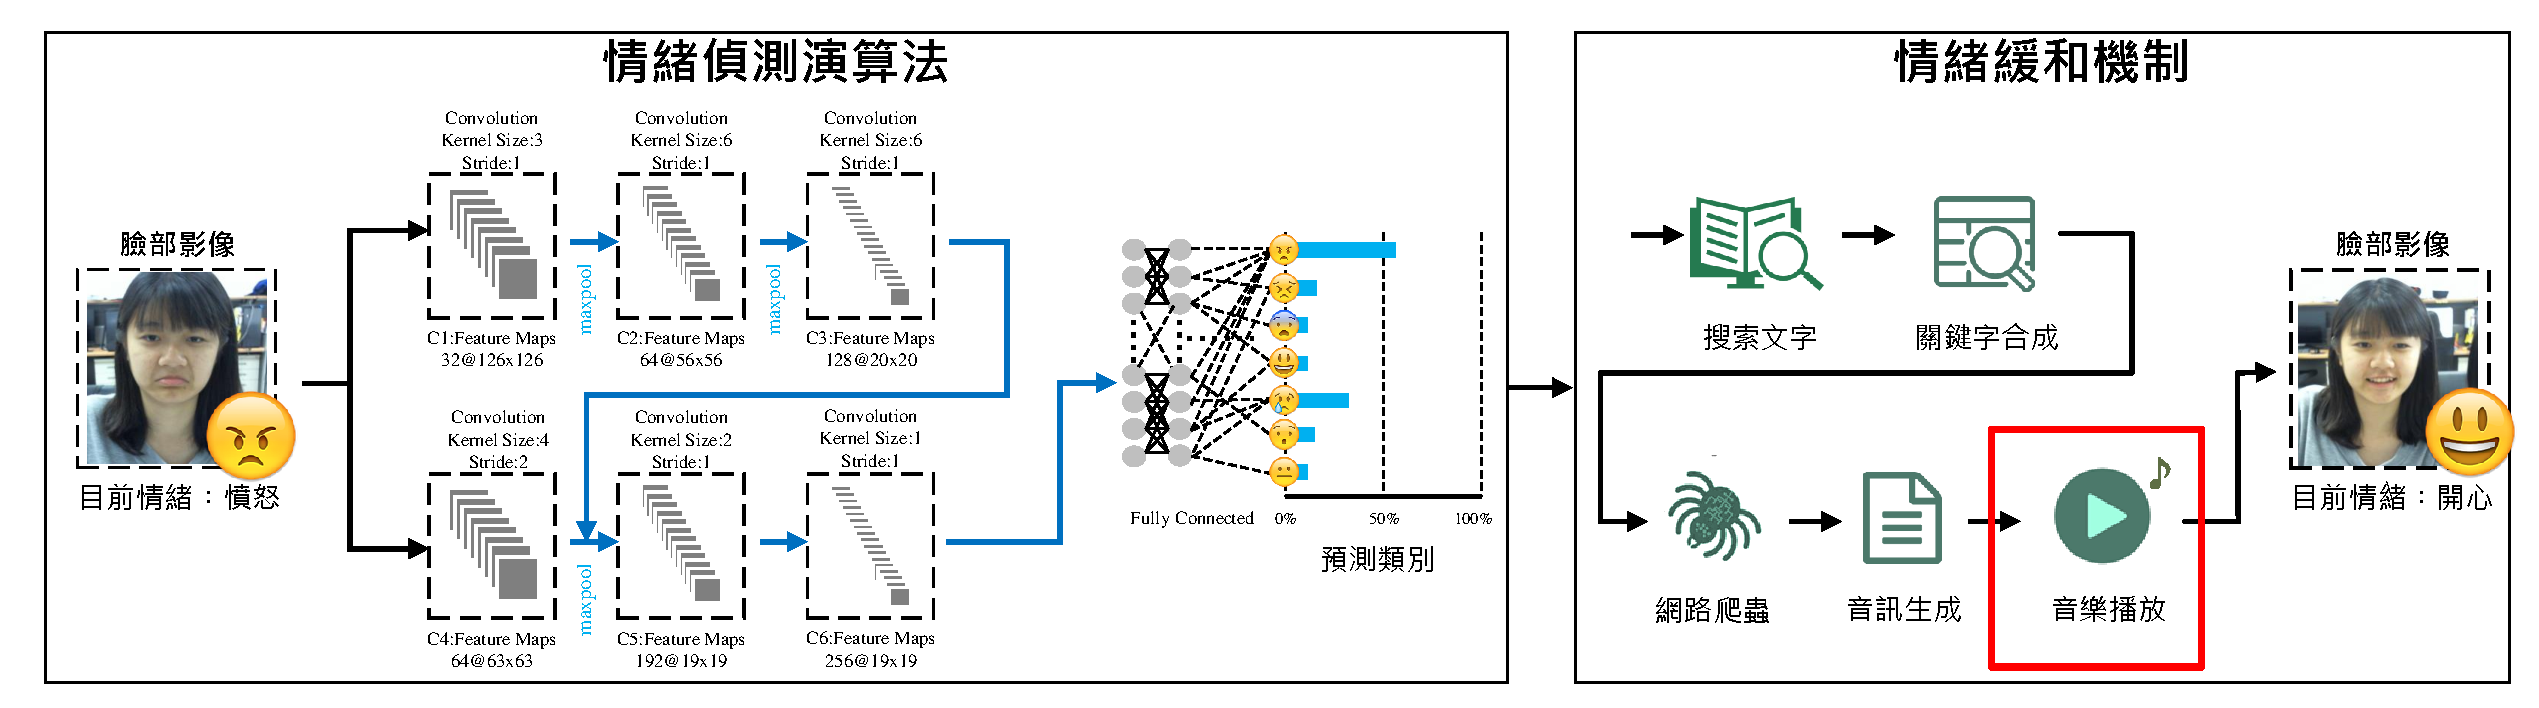
\includegraphics[width=5cm]{./Figures/framework8.pdf}
\end{flushright}
\end{figure}

\vspace{-5mm}

\begin{itemize}
\item \Large播放文字及音樂緩和情緒
\end{itemize}

\begin{figure}[!t]
\begin{center}
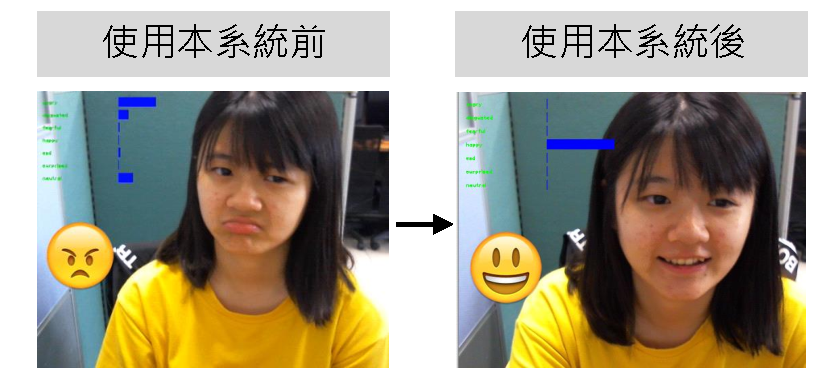
\includegraphics[width=11cm]{./Figures/result.pdf}
\end{center}
\end{figure}
\end{frame}

\begin{frame}
\frametitle{作品介紹}
%伺服器端
\begin{itemize}
\item \Large伺服器端
\end{itemize}

\begin{figure}[!t]
\begin{center}
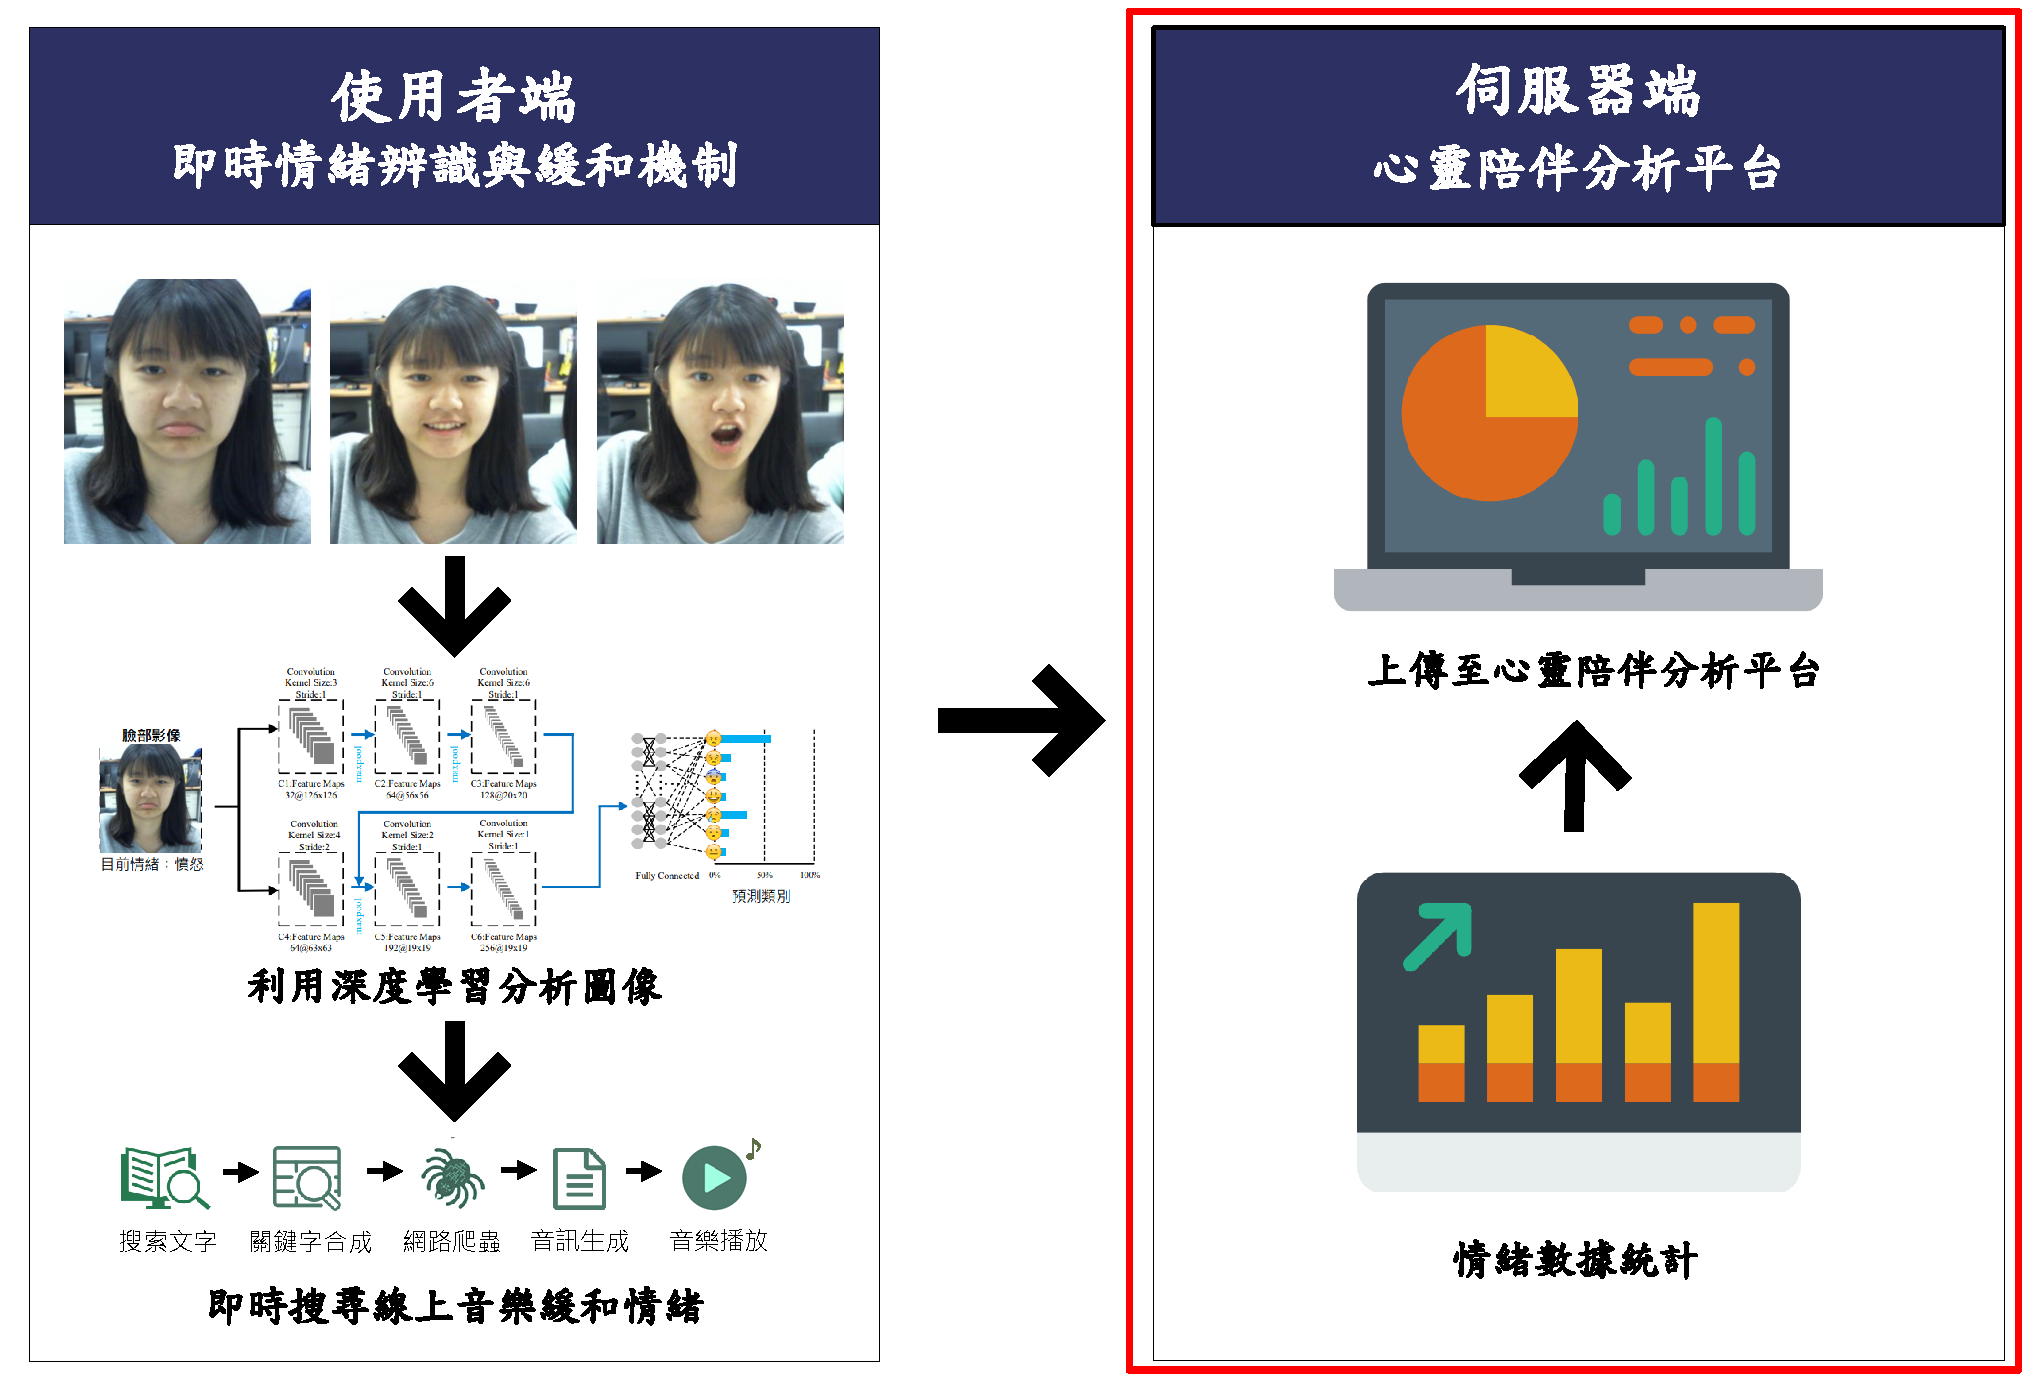
\includegraphics[width=9.4cm]{./Figures/UserAndServer2.pdf}
\end{center}
\end{figure}

\end{frame}

\begin{frame}
\frametitle{作品介紹}
%分析
\begin{itemize}
\item \Large伺服器端
\end{itemize}
\begin{itemize}
\item[-]  呈現介面 : 情緒統計、小建議、聊聊功能\\
\end{itemize}
\vspace{-3mm}

\begin{figure}[!t]
\begin{center}
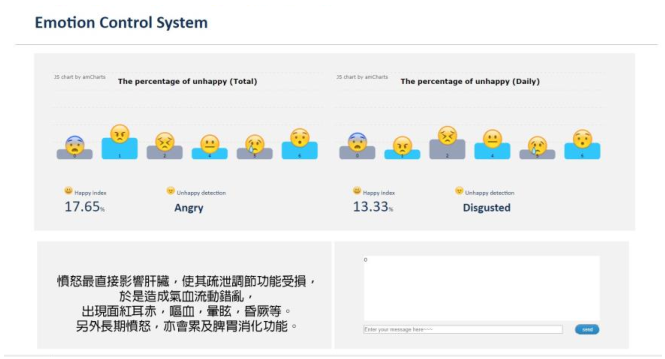
\includegraphics[width=9.7cm]{./Figures/web.pdf}
\end{center}
\end{figure}

\end{frame}

\begin{frame}
\frametitle{作品介紹}
%情緒統計
\begin{itemize}
\item \Large情緒統計
\end{itemize}

\begin{figure}[!t]
\begin{center}
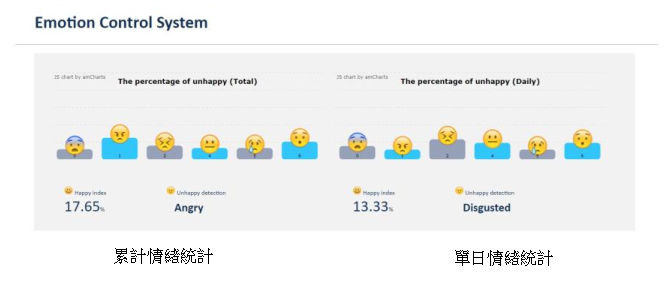
\includegraphics[width=9.7cm]{./Figures/web2.pdf}
\end{center}
\end{figure}

\end{frame}

\begin{frame}
\frametitle{作品介紹}
%情緒統計
\begin{itemize}
\item \Large 小建議
\end{itemize}

\begin{figure}[!t]
\begin{center}
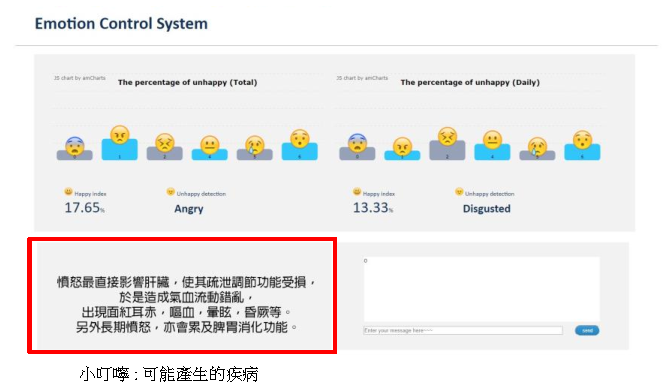
\includegraphics[width=9.7cm]{./Figures/web3.pdf}
\end{center}
\end{figure}

\end{frame}

\begin{frame}
\frametitle{作品介紹}
%情緒統計
\begin{itemize}
\item \Large 聊聊功能
\end{itemize}

\begin{figure}[!t]
\begin{center}
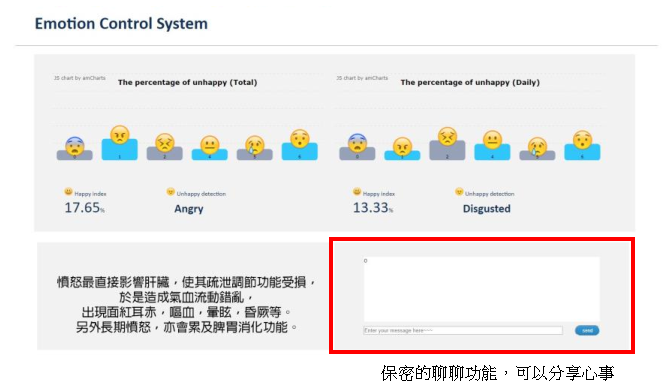
\includegraphics[width=9.7cm]{./Figures/web4.pdf}
\end{center}
\end{figure}

\end{frame}

\section{實機測試}

\begin{frame}
\frametitle{實機測試}
%負面情緒

\vspace{-5mm}
\begin{figure}[t]
\begin{center}
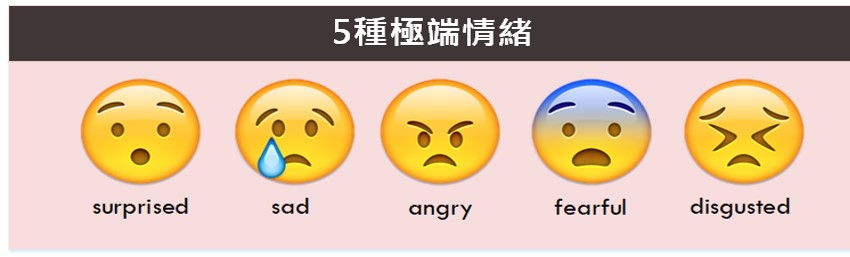
\includegraphics[width=8cm]{./Figures/508.jpg}
\end{center}
\end{figure}

\vspace{5mm}
\begin{figure}[!t]
\begin{center}
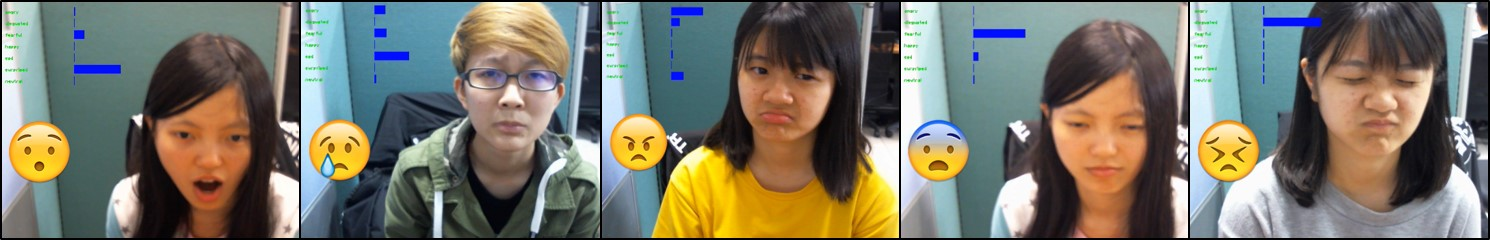
\includegraphics[width=12cm]{./Figures/509.jpg}
\end{center}
\end{figure}

\end{frame}

\begin{frame}
\frametitle{實機測試}
%正面情緒

%\vspace{-5mm}
\begin{figure}[t]
\begin{center}
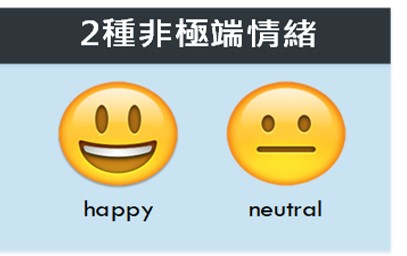
\includegraphics[width=4cm]{./Figures/510.jpg}
\end{center}
\end{figure}

\vspace{3mm}
\begin{figure}[!t]
\begin{center}
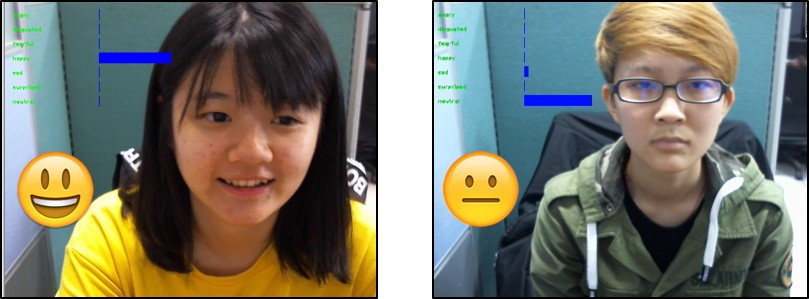
\includegraphics[width=8cm]{./Figures/511.jpg}
\end{center}
\end{figure}

\end{frame}

\section{總結}

\begin{frame}
\frametitle{總結}
\begin{itemize}
\item\Large基於即時情緒分析之心靈陪伴系統
\end{itemize}

\begin{columns}
\column{.5\textwidth}
\begin{itemize}
\item[-] \Large\bf 即時分析情緒
\vspace{5mm}
\item[-] \Large\bf 專業的緩和機制
\vspace{5mm}
\item[-] \Large\bf 後端平台做分析追蹤
\end{itemize}

\column{.5\textwidth}
\begin{figure}[!t]
\begin{flushright}
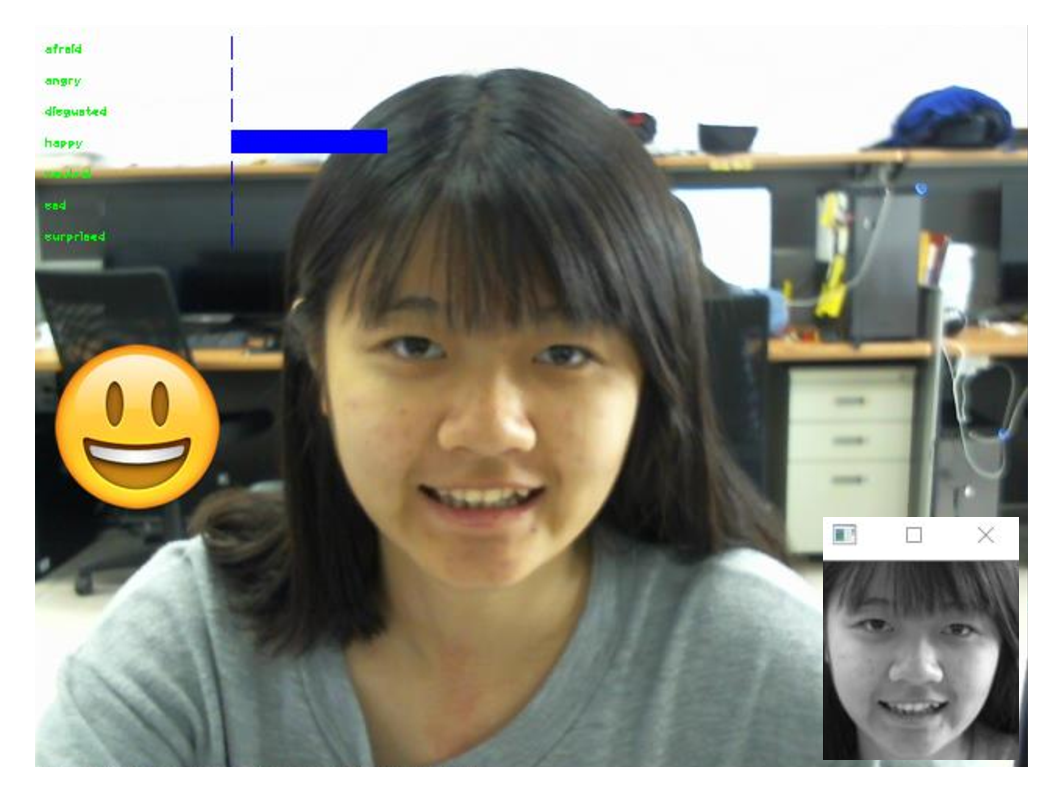
\includegraphics[width=0.9\textwidth]{Figures/DetectResult.pdf}
\end{flushright}
\end{figure}
\end{columns}

\end{frame}

\begin{frame}
\frametitle{總結}
\begin{itemize}
\item\Large基於即時情緒分析之心靈陪伴系統
\end{itemize}
\begin{itemize}
\item[\Large\bf \textcolor{red}v] \Large\bf Relevance and validity of theme
\end{itemize}
\begin{itemize}
\item[-]  Machine to human
\item[-]  Human to machine
\end{itemize}

\begin{itemize}
\item[\Large\bf \textcolor{red}v] \Large\bf Design concept
\end{itemize}
\begin{itemize}
\item[-]  使用方式簡易\\
\textcolor{red}{可行性高}
\item[-]  具有重複性、即時性、專業性\\
\textcolor{red}{創新創意}
\end{itemize}
\end{frame}

\begin{frame}
\frametitle{總結}
\begin{itemize}
\item\Large基於即時情緒分析之心靈陪伴系統
\end{itemize}
\begin{itemize}
\item[\Large\bf \textcolor{red}v] \Large\bf User experience
\end{itemize}
\begin{itemize}
\item[-]  介面簡單易懂
\item[-]  伺服器端清楚明瞭
\end{itemize}

\begin{itemize}
\item[\Large\bf \textcolor{red}v] \Large\bf Overall design progress
\end{itemize}
\begin{itemize}
\item[-]  documentation \textcolor{red}{~100\%}
\item[-]  demonstrations \textcolor{red}{100\%}
\item[-]  presentation     \textcolor{red}{~~~~~100\%}
\end{itemize}
\end{frame}

\end{CJK}
\end{document}

